% !Mode:: "TeX:UTF-8"
%%%%%%%%%%%%%%%%%%%%%%%%%%%%%%%%%%%%%%%%%%%%%%%%%%%%%%%%%%%%%%%%%%%%%%%%%%%%%%%%
%          ,
%      /\^/`\
%     | \/   |                CONGRATULATIONS!
%     | |    |             SPRING IS IN THE AIR!
%     \ \    /                                                _ _
%      '\\//'                                               _{ ' }_
%        ||                     hithesis v3                { `.!.` }
%        ||                                                ',_/Y\_,'
%        ||  ,                   dustincys                   {_,_}
%    |\  ||  |\          Email: yanshuoc@gmail.com             |
%    | | ||  | |            https://yanshuo.name             (\|  /)
%    | | || / /                                               \| //
%    \ \||/ /       https://github.com/dustincys/hithesis      |//
%      `\\//`   \\   \./    \\ /     //    \\./   \\   //   \\ |/ /
%     ^^^^^^^^^^^^^^^^^^^^^^^^^^^^^^^^^^^^^^^^^^^^^^^^^^^^^^^^^^^^^^
%%%%%%%%%%%%%%%%%%%%%%%%%%%%%%%%%%%%%%%%%%%%%%%%%%%%%%%%%%%%%%%%%%%%%%%%%%%%%%%%
\documentclass[fontset=fandol,type=bachelor,campus=weihai]{hithesisbook}
% 此处选项中不要有空格
%%%%%%%%%%%%%%%%%%%%%%%%%%%%%%%%%%%%%%%%%%%%%%%%%%%%%%%%%%%%%%%%%%%%%%%%%%%%%%%%
% 必填选项
% type=doctor|master|bachelor|postdoc
%%%%%%%%%%%%%%%%%%%%%%%%%%%%%%%%%%%%%%%%%%%%%%%%%%%%%%%%%%%%%%%%%%%%%%%%%%%%%%%%
% 选填选项(选填选项的缺省值已经尽可能满足了大多数需求,除非明确知道自己有什么
% 需求)
% campus=shenzhen|weihai|harbin
%   含义:校区选项,默认harbin
% glue=true|false
%   含义:由于我工规范中要求字体行距在一个闭区间内,这个选项为true表示tex自
%   动选择,为false表示区间内一个最接近版心要求行数的要求的默认值,缺省值为
%   false。
% tocfour=true|false
%   含义:是否添加第四级目录,只对本科文科个别要求四级目录有效,缺省值为
%   false
% fontset=windows|mac|ubuntu|fandol|adobe
%   含义:设置字体,若不指定会自动识别系统,然后设置字体。fandol是开源字体,自行
%   下载安装后设置使用。windows是中易字库,窝工默认常用字体,绝对没毛病。mac和
%   ubuntu 默认分别是华文和思源字库,理论上用什么字库都行。后两种字库的安装方法
%   到谷歌上百度一下什么都有了。Linux非ubuntu发行版、非x86架构机器等如何运行可到
%   github issue上讨论。
% tocblank=true|false
%   含义:目录中第一章之前,是否加一行空白。缺省值为true。
% chapterhang=true|false
%   含义:目录的章标题是否悬挂居中,规范中要求章标题少于15字,所以这个选项
%   有无没什么用,除了特殊需求。缺省值为true。
% fulltime=true|false
%   含义:是否全日制,缺省值为true。非全日制如同等学力等,要在cover中设置类
%   型,封面中不同格式
% subtitle=true|false
%   含义:论文题目是否含有副标题,缺省值为false,如果有要在cover中设置副标
%   题内容,封面中显示。
% newgeometry=one|two|no
%   含义:规范中的自相矛盾之处,版芯是否包含页眉页脚,旧方法是按照包含页眉
%   页脚来设置。该选项是多选选项,如果设置为no,则版新为旧模板的版芯设置方法,
%   如果设置该选项one或two,分别对应两种页眉页码对应版芯线的相对位置。第一种
%   是严格按照规范要求,难看。第二种微调了页眉页码位置,好一点。默认two。
% debug=true|false
%   含义:是否显示版芯框和行号,用来调试。默认否。
% openright=true|false
%   含义:博士论文是否要求章节首页必须在奇数页,此选项不在规范要求中,按个
%   人喜好自行决定。 默认否。注意,窝工的默认情况是打印版博士论文要求右翻页
%   ,电子版要求非右翻页且无空白页。如果想DIY(或身不由己DIY)在什么地方右
%   翻页,将这个选项设置为false,然后在目标位置添加`\cleardoublepage`命令即
%   可。
% library=true|false
%   含义:是否为提交到图书馆的电子版。默认否。注意:如果设置成true,那么
%   openright选项将被强制转换为false。
% capcenterlast=true|false
%   含义:图题、表题最后一行是否居中对齐(我工规范要求居中,但不要求居中对
%   齐),此选项不在规范要求中,按个人喜好自行决定。默认否。
% subcapcenterlast=true|false
%   含义:子图图题最后一行是否居中对齐(我工规范要求居中,但不要求居中对齐
%   ),此选项不在规范要求中,按个人喜好自行决定。默认否。
% absupper=true|false
%   含义:中文目录中的英文摘要在中文目录中的大小写样式歧义,在规范中要求首
%   字母大写,在work样例中是全大写。该选项控制是否全大写。默认否。
% bsmainpagenumberline=true|false
%   含义:由于本科生论文官方模板的页码和页眉格式混乱,提供这个选项自定义设
%   置是否在正文中显示页码横线,默认显示。
% bsfrontpagenumberline=true|false
%   含义:由于本科生论文官方模板的页码和页眉格式混乱,提供这个选项自定义设
%   置是否在前文中显示页码横线,默认显示。
% bsheadrule=true|false
%   含义:由于本科生论文官方模板的页码和页眉格式混乱,提供这个选项自定义设
%   置是否显示页眉横线,默认显示。
% splitbibitem=true|false
%   含义:参考文献每一个条目内能不能断页,应广大刀客要求添加。默认否。
% newtxmath=true|false
%   含义:数学字体是否使用新罗马。默认是。
% chapterbold=true|false
%   含义:本科生章标题在目录和正文中是否加粗
% engtoc=true|false
%   含义:非博士生需要添加英文目录的,手动添加,如果是博士,此开关无效
% zijv=word|regu
%   含义:字距设置为规范规定33个字还是word中34个字。默认regu。
%%%%%%%%%%%%%%%%%%%%%%%%%%%%%%%%%%%%%%%%%%%%%%%%%%%%%%%%%%%%%%%%%%%%%%%%%%%%%%%%
\usepackage{hithesis}
\usepackage{pdfpages}
\usepackage{float}
\usepackage{enumitem}
\usepackage{listings}
\lstset {
    basicstyle          =   \sffamily,          % 基本代码风格
    keywordstyle        =   \bfseries,          % 关键字风格
    commentstyle        =   \rmfamily\itshape,  % 注释的风格,斜体
    stringstyle         =   \ttfamily,  % 字符串风格
    flexiblecolumns,                % 别问为什么,加上这个
    numbers             =   left,   % 行号的位置在左边
    showspaces          =   false,  % 是否显示空格,显示了有点乱,所以不现实了
    numberstyle         =   \zihao{-5}\ttfamily,    % 行号的样式,小五号,tt等宽字体
    showstringspaces    =   false,
    captionpos          =   t,      % 这段代码的名字所呈现的位置,t指的是top上面
    frame               =   lrtb,   % 显示边框
    }
\setlist[itemize]{itemsep=1pt}
\graphicspath{{figures/}}


\begin{document}
\frontmatter
% !Mode:: "TeX:UTF-8"

\hitsetup{
  %******************************
  % 注意:
  %   1. 配置里面不要出现空行
  %   2. 不需要的配置信息可以删除
  %******************************
  %
  %=====
  % 秘级
  %=====
  statesecrets={公开},
  natclassifiedindex={TM301.2},
  intclassifiedindex={62-5},
  %
  %=========
  % 中文信息
  %=========
  ctitleone={基于卡尔曼滤波器的},%本科生封面使用
  ctitletwo={多目标追踪预测算法},%本科生封面使用
  ctitlecover={基于卡尔曼滤波器的多目标追踪预测算法},%放在封面中使用,自由断行
  ctitle={基于卡尔曼滤波器的多目标追踪预测算法},%放在原创性声明中使用
  % csubtitle={一条副标题}, %一般情况没有,可以注释掉
  cxueke={工学},
  csubject={机器人工程},
  caffil={海洋工程学院},
  cauthor={朱纹轩},
  csupervisor={赵明航副教授},
  cassosupervisor={某某某教授}, % 副指导老师
  ccosupervisor={某某某教授}, % 联合指导老师
  % 日期自动使用当前时间,若需指定按如下方式修改:
  cdate={2023年5月27日},
  cstudentid={2191300231},
  cstudenttype={学术学位论文}, %非全日制教育申请学位者
  cnumber={no9527}, %编号
  cpositionname={哈铁西站}, %博士后站名称
  cfinishdate={20XX年X月---20XX年X月}, %到站日期
  csubmitdate={20XX年X月}, %出站日期
  cstartdate={3050年9月10日}, %到站日期
  cenddate={3090年10月10日}, %出站日期
  %(同等学力人员)、(工程硕士)、(工商管理硕士)、
  %(高级管理人员工商管理硕士)、(公共管理硕士)、(中职教师)、(高校教师)等
  %
  %
  %=========
  % 英文信息
  %=========
  etitle={Research on key technologies of partial porous externally pressurized gas bearing},
  esubtitle={This is the sub title},
  exueke={Engineering},
  esubject={Computer Science and Technology},
  eaffil={\emultiline[t]{School of Mechatronics Engineering \\ Mechatronics Engineering}},
  eauthor={Yu Dongmei},
  esupervisor={Professor XXX},
  eassosupervisor={XXX},
  % 日期自动生成,若需指定按如下方式修改:
  edate={December, 2017},
  estudenttype={Master of Art},
  %
  % 关键词用“英文逗号”分割
  ckeywords={全局快门, 卷积神经网络, 卡尔曼滤波, 多目标追踪},
  ekeywords={global shutter, convolutional neural network, kalman filter, multi-target tracking},
}

\begin{cabstract}
  本文提出了一种基于卡尔曼滤波器的多目标追踪预测算法。
  在相机选型方面,选择了全局快门方式、高帧率的相机以提高检测动态目标的能力;
  在主从机时间帧对齐方面,基于通信设计了动态时间帧对齐,保证了主从机使用同一时钟源;
  在目标检测算法方面,采用了将传统数字图像处理与深度学习相结合的方案,
  能够高效准确地检测到复杂光照环境下的目标;
  在运动预测算法方面,
  使用了基于卡尔曼滤波器的运动模型,对目标的位置和速度进行预测;
  在追踪算法方面,使用了类贪心算法的多目标追踪算法,
  提高追踪的准确性和效率。实验结果表明,本算法能够高效准确地完成多目标追踪预测任务,并且具有较高的实时性和鲁棒性。
\end{cabstract}

\begin{eabstract}
  This article proposes a multi-target tracking 
  and prediction algorithm based on the Kalman filter. 
  In terms of camera selection, 
  cameras with a global shutter mode and high frame rates 
  were chosen to improve the ability to detect dynamic targets. 
  For master-slave time frame alignment, 
  dynamic time frame alignment based on communication was designed to ensure that the master and slave machines use the same clock source. In terms of target detection algorithm, a combination of traditional digital image processing and deep learning was adopted to efficiently and accurately detect targets in complex lighting environments. For motion prediction algorithm, a motion model based on the Kalman filter was used to predict the position and velocity of the target. For tracking algorithm, a multi-target tracking algorithm based on a greedy-like algorithm was used to improve tracking accuracy and efficiency. Experimental results show that this algorithm can efficiently and accurately complete multi-target tracking and prediction tasks, and has high real-time performance and robustness.
\end{eabstract}
 % 封面
\makecover
% \begin{denotation}
\begin{table}[h]%此处最好是h
\caption{国际单位制中具有专门名称的导出单位}
\vspace{0.5em}\centering\wuhao
\begin{tabular}{ccccc}
\toprule[1.5pt]
量的名称&单位名称&单位符号&其它表示实例\\
\midrule[1pt]
频率&赫[兹]&Hz&s-1\\
\bottomrule[1.5pt]
\end{tabular}
\end{table}
\end{denotation}
%物理量名称表,符合规范为主,有要求添加
\tableofcontents %目录
\mainmatter
% !Mode:: "TeX:UTF-8"

\chapter[绪论]{绪论}[Harbin Institute of Technology Postgraduate Dissertation Writing Specifications]

\section{课题背景及研究目的和意义}[Content specification]

本研究基于全国大学生机器人大赛RoboMaster,
旨在为战队研发一种高效鲁棒的自动瞄准算法,
实现对装甲板的识别、坐标解算、运动建模、预测等算法。
一键瞄准、自动锁定,帮助操作手提高弹丸击打装甲板的命中率,从而取得比赛的胜利。
同时,该研究涉及大量的机器人领域的理论知识,
并涉及实际的工程开发。学以致用,提高对专业领域知识的掌握程度。

\section{研究现状}

\subsection{目标检测算法研究现状}
目标检测是计算机视觉领域中的一项重要任务,旨在从图像或视频中检测出目标物体的位置和类别。
目标检测算法的研究一直是计算机视觉领域的热点之一。
目前,主要的目标检测算法可以分为两类:基于传统机器学习方法的算法和基于深度学习方法的算法。\par


传统机器学习方法主要包括特征提取和分类两个步骤。
常用的特征提取算法有方向梯度直方图(Histogram of Oriented Gradient, HOG)特征\cite{pang2011efficient}和尺度不变特征转换(Scale-invariant feature transform, SIFT)特征\cite{ng2003sift}等。
其中,HOG特征主要用于行人检测,SIFT特征主要用于物体检测。
分类算法主要包括自适应增强(Adaptive Boosting, Adaboost)\cite{hastie2009multi}、支持向量机(Support Vector Machine, SVM)\cite{schuldt2004recognizing}和随机森林(Random Forest, RF)\cite{biau2016random}等。
这些算法在一定程度上可以实现目标检测,但是它们的检测效果和速度相对较低,已经逐渐被深度学习算法所替代。

\par

随着深度学习算法的发展,基于深度学习的目标检测算法逐渐成为主流。
常用的深度学习模型包括快速区域卷积神经网络(Faster Region-based Convolutional Neural Network, Fast R-CNN)\cite{girshick2015fast}、基于单次检测的目标检测算法(You Only Look Once, YOLO)\cite{jiang2022review}等。
这些算法在目标检测准确率和速度上都有很大的提升,已经广泛应用于各个领域,例如自动驾驶、安防监控、医疗诊断等。
\par
此外,当前目标检测算法研究的重点主要集中在以下几个方面:
\begin{itemize}[itemindent=2em]
    \item 目标检测算法的精度和速度的平衡问题,通常称为精度-速度权衡(trade-off)。
    这是因为在目标检测任务中,算法需要同时实现高精度的目标定位和分类,同时保持较快的处理速度。
    在追求更高精度的同时,算法可能需要更复杂的模型和更多的计算资源。
    这可能导致算法的处理速度变慢,不适用于实时应用或大规模数据集的处理。
    相反,追求更快的处理速度可能会牺牲一定的精度,导致错误的目标检测或较低的定位精度。
    
    \item 目标检测算法的可解释性问题,即如何让算法输出的检测结果更容易被人理解和解释。
    目标检测算法的可解释性问题指的是对算法内部决策和输出结果的解释和理解能力。
    在某些应用场景中,仅仅依靠算法的高准确率可能是不够的,还需要能够理解算法是如何做出决策的、
    哪些特征导致了目标的检测等。这对于一些对决策过程有强解释需求的应用领域尤其重要,
    比如医疗诊断、自动驾驶等。
    
    \item 小样本目标检测,即在少量样本的情况下实现准确的目标检测,这对于一些特定领域的应用非常重要。以下是关于小样本目标检测的一些研究热点:
    迁移学习和预训练模型\cite{zhuang2020comprehensive}:迁移学习使用在大规模数据集上预训练的模型作为初始权重,并通过微调或其他适应性方法来调整模型以适应小样本目标检测任务。预训练模型,可以提供在大规模数据上学习的通用特征,从而加快在小样本数据上的学习。
    元学习\cite{hospedales2021meta}:元学习(或称为学习到学习)是一种可以在小样本情况下进行目标检测的方法。通过在大量不同任务上进行训练,元学习模型可以学习到一种学习策略,可以快速适应新任务。
    生成对抗网络(Generative Adversary Network, GAN):生成对抗网络可以通过生成逼真的合成样本来增强小样本目标检测任务的训练。
    具有注意力机制的模型:注意力机制可以帮助模型关注关键区域,从而在小样本目标检测任务中提升性能。
    
    \item 目标检测算法在复杂场景下的应用,例如低光照、遮挡、姿态变化等情况下的检测效果如何提升。
    
\end{itemize}


总之,目标检测算法的研究还有很大的发展空间,未来的研究方向将更加注重模型的实用性和鲁棒性,以满足实际应用的需求。

\subsection{卡尔曼滤波器研究现状}
卡尔曼滤波器是一种经典的状态估计方法,可用于估计时间序列的未知状态。在目标跟踪、自动导航和机器人等领域中得到广泛应用。目前,卡尔曼滤波器的研究现状主要包括以下几个方面:
\par
卡尔曼滤波器的基础理论。
卡尔曼滤波器的基础理论已经相对成熟,包括线性系统、高斯噪声和线性状态估计等方面的理论研究,
这些理论为卡尔曼滤波器的应用提供了坚实的基础。
\par
卡尔曼滤波器的改进和优化。
为了提高卡尔曼滤波器的估计精度和稳定性,一些改进和优化方法被提出:
扩展卡尔曼滤波器(Extended Kalman Filter, EKF)\cite{ribeiro2004kalman}是对非线性系统进行状态估计的扩展。它通过在非线性函数上进行泰勒级数展开,将非线性系统近似为线性系统,从而应用线性卡尔曼滤波器的方法。扩展卡尔曼滤波器在非线性系统的状态估计中得到广泛应用,并且已经成为卡尔曼滤波器的标准扩展之一。
无迹卡尔曼滤波器(Unscented Kalman Filter, UKF)\cite{wan2000unscented}是对扩展卡尔曼滤波器的改进,旨在提高非线性系统的状态估计精度。它通过选择一组特定的采样点(称为无迹变换)来近似非线性系统的均值和协方差。无迹卡尔曼滤波器相比于扩展卡尔曼滤波器在非线性系统估计方面具有更好的稳定性和准确性。
粒子滤波器(Particle Filter,PF)\cite{gustafsson2010particle}基于贝叶斯滤波理论,通过使用一组粒子来表示状态的后验概率分布。每个粒子都代表了系统状态的一个假设或样本。粒子的权重表示了该假设的后验概率。粒子滤波器通过递归地更新粒子的权重和位置,来逼近并估计系统的后验概率分布。
这些方法使卡尔曼滤波器能够更好地适应非线性系统和非高斯噪声的情况,
并取得了一定的效果。

\subsection{多目标追踪研究现状}
多目标追踪预测算法是指在视频或图像序列中,对多个目标的轨迹进行跟踪和预测的算法。
目前,多目标追踪预测算法的研究主要集中在以下几个方面:
\par
基于传统方法的算法。
传统的多目标追踪算法主要包括卡尔曼滤波器、粒子滤波器、条件随机场和蒙特卡罗方法等。
这些算法在目标跟踪和预测中有着广泛的应用,但是在处理复杂场景和高速移动目标时,精度和效率存在一定的限制。
\par
基于深度学习方法的算法。
深度学习方法在多目标追踪预测算法中也有广泛的应用\cite{xu2019deep},
比如深度排序追踪器(Deep Learning to Track with Sorting, Deep SORT)\cite{wojke2017simple}等。
这些算法主要利用深度学习网络进行目标检测和特征提取,并使用各种跟踪方法进行目标跟踪和预测。
例如,Deep SORT使用卷积神经网络来提取目标特征,并使用传统的匈牙利算法来关联跟踪器。
这些算法的优势在于准确率高、鲁棒性好,但是计算量大,处理速度相对较慢。
\par
融合感知模态的多目标追踪:多模态感知融合是另一个研究热点,旨在利用多个传感器(如摄像头、激光雷达、雷达等)提供的信息来改进多目标追踪性能。通过融合不同传感器的数据,可以提高目标检测和跟踪的鲁棒性,并增强对目标的理解和描述。
\par
端到端的多目标追踪:近年来,出现了一些基于深度学习的端到端多目标追踪方法。这些方法将目标检测、特征提取和目标关联等任务整合到一个网络中,通过联合训练来直接优化多目标追踪的性能。端到端的方法具有简化流程、减少计算复杂性和提高整体性能等优点。

\section{本文的主要研究内容}
本文的研究内容包括以下几点:
\begin{itemize}[itemindent=2em]
    \item 基于RoboMaster比赛环境的工业相机选型。
    \item 基于通信的主从机时钟对齐。
    \item 将传统数字图像处理技术与深度学习相结合的目标检测算法。
    \item 基于卡尔曼滤波器的运动物体建模、预测算法。
    \item 基于物体运动模型的多目标追踪算法。
    \item 受空气阻力的弹道迭代计算方法。
\end{itemize}






% 

\chapter[相机选型与基本设置]{相机选型与基本设置}[Harbin Institute of Technology Postgraduate Dissertation Writing Specifications]

\section{引言}[Content specification]
相机是计算机视觉中非常重要的一部分,负责获取环境中的图像信息,为后续的图像处理和算法提供输入数据。
因此,在进行计算机视觉项目时,选择适合的相机和合理的相机参数设置是非常关键的。

\section{相机选型}[Content specification]
尽量选择高帧率、感光片大的相机,在此基础上选择光圈大的镜头,焦距选择视情况而定。
下面详细阐述:\par

\begin{itemize}[itemindent=2em]
    \item 分辨率:一般分辨率越高,图像质量越好,越有利于识别算法和测距算法。但分辨率越高,图像最大采集帧率越低,
    且检测算法耗时增加,价格也相应越高。因此选择分辨率在30万到100万像素的相机即可。
    \item 帧率:帧率越高,运动图像捕捉能力越好。由于我们需要检测高速移动或者旋转的目标,因此帧率越高越好。
    根据应用场景需要捕捉的运动速度和动态要求,选择适合的帧率。
    \item 传感器尺寸和类型:CMOS和CCD是现代数字图像传感器的两种常见类型。
    CMOS传感器具有低功耗、低噪声、高帧率等优点,且质量更小,所以选择CMOS相机。
    \item CMOS传感器有两种快门方式,卷帘快门和全局快门。
    全局快门曝光时间更短,但噪声更大;卷帘快门可以达到更高的帧速,但当
    曝光时间较长或物体移动较快时产生果冻效应。
    为了适应RoboMaster比赛场景的需求,选择全局快门的相机。
    \item 工作温度和防护等级:根据应用环境和需求,选择适合的工作温度和防护等级。
    工业相机一般需要在恶劣环境下工作,如高温、灰尘等,所以防护等级要求较高。
    \item 软件支持:算法运行环境为Linux,
    工业相机的软件平台需要支持图像处理和数据分析等功能,
    通常需要与特定的软件开发工具包配合使用,且售后的技术支持和SDK软件包的是否适合二次开发也是重点。

\end{itemize}


一张成像清晰、亮度均匀的图片非常有利于后续的图像处理算法,因此如何设置相机参数,以及如何预处理原始图像后都非常重要。
\section{相机硬件设置}[Content specification]
拿到相机后,基本设置如下:将光圈拧到最大;调整成像平面与光心的距离,使得5m成像最清晰;涂抹螺丝胶,防止相机在剧烈震动的情况下因螺丝松动而成像不清。之所以将光圈拧到最大,是为了在达到相同图像亮度的情况下获得更短的曝光时间,进而提高相机帧率。
\section{相机软件设置}[Content specification]
模拟增益调高,目的:一是在达到相同图像亮度的情况尽可能减少曝光时间从而提高取图帧率,
不过由于增益拉高后图像噪点也会增加,因此需要平衡; 
二是使得发光体在图像中更加明显,从而二值化阈值可以取到非常高,可以防止过曝给灯条的提取造成影响,
因为即使在过曝的情况下,光晕的灰度值与真正的发光体还是有较大的区别,通过高阈值筛选可以很好的提取灯条。

设置相机白平衡参数,使得成像色彩正常,
迈德威视相机的软件工具包提供了自动调节白平衡参数的功能,只需要将相机对准白色物体,
然后点击“白平衡”按钮即可。

\section{本章小结}[Content specification]
本章主要介绍了相机选型、硬件设置和软件设置等方面的知识。
在相机选型方面,需要考虑分辨率、帧率、传感器尺寸和类型、工作温度和防护等级、
以及软件支持等因素。在硬件设置方面,需要注意光圈的设置和成像平面与光心的距离等。
在软件设置方面,需要注意模拟增益的调整和颜色通道增益的选择等。
明确这些方面的知识,可以使相机的使用更加得心应手,也能够为后续的图像处理和算法提供更好的输入数据。

% \chapter[主从机时钟对齐]{主从机时钟对齐}[Harbin Institute of Technology Postgraduate Dissertation Writing Specifications]

\section{引言}[Content specification]
在工业自动化和嵌入式系统中,上位机和下位机之间的时间同步是非常重要的。通常,下位机的时间通常是由硬件时钟提供的,
而上位机的时间通常是由操作系统提供的。由于硬件时钟和操作系统时钟存在不同步的可能,
因此需要基于通信方法来同步它们的时间。\par

\section{通信时延测量}[Content specification]
对于一固定的装甲板,晃动云台,则理论上结算的装甲板在惯性系下的坐标应该是不变的。
然而,由于通信时延、相机成像时间误差、计时精度、陀螺仪数据精度与系统偏差等因素,
不可能精确的获得的图像对应的陀螺仪数据。这里面影响因素最大的就是通信时延,因此通过调节通信时延量,
使得惯性系下的装甲板坐标晃动幅度最后,此时得到的通信时延量认为是真实的通信时延。
\par
图\ref{delay}展示了在通信时延量在超前、滞后、大致准确时解算的装甲板在惯性下的坐标。
\begin{figure}[H]
    \centering
    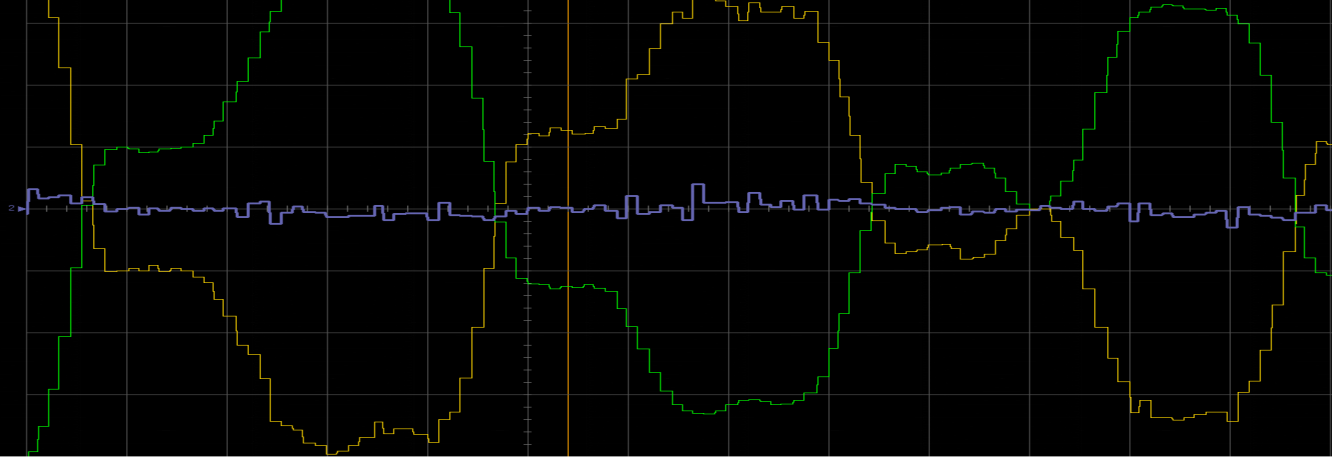
\includegraphics[width=.8\textwidth]{delay.png} 
    \caption{不同通信时延对应的装甲板惯性下的坐标} 
    \label{delay}
\end{figure}

\section{动态时间帧对齐}[Content specification]

基本思想如下:事先通过技术手段测量通信时延。然后以下位机的时钟为基准,下位机定频向上位机发送本机的时钟信息,上位机将计算本机时钟与下位机时钟之差(在考虑通信时延的情况下),
并将数据放入到循环队列中,当需要在上位机获取下位机时钟时刻时,
通过计算循环队列的平均值作为上下位机时钟偏移量加到本机时钟就可以获得下位机的时钟时刻,如图\ref{clock_sync}所示。

\begin{figure}[H]
    \centering
    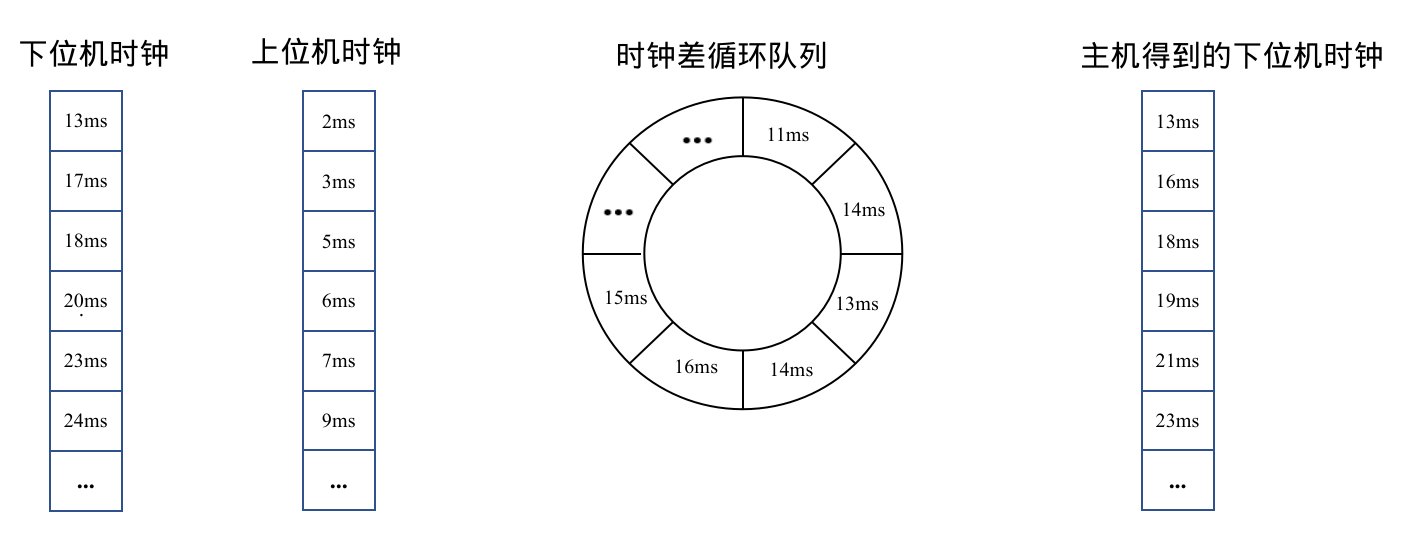
\includegraphics[width=.8\textwidth]{clock_sync.png} 
    \caption{自实现时钟同步} 
    \label{clock_sync}
\end{figure}

% \subsection{线程安全的时间队列}[Content specification]








\section{本章小结}[Content specification]
通过观测固定装甲板惯性下的坐标浮动情况测量通信时延,基于通信实现动态上下位机时间帧对齐,
实现了双机时钟的统一,有利于后续的坐标转换、云台姿态控制等。







% !Mode:: "TeX:UTF-8"

\chapter[目标检测算法设计]{目标检测算法设计}[Harbin Institute of Technology Postgraduate Dissertation Writing Specifications]



\section{引言}[Content specification]

目标检测是目标追踪的前提,对于目标检测来说,我们要求它运行速度快,目标召回率与正确率高。
尽管基于深度学习端到端的方案是目前实现成本最低的方案,但是由于计算设备TX2的GPU性能性能较弱,全图推理时间较长(实际测试约为50fps),遂放弃。
\par
本章创新性地提出了一种将传统数字图像处理算法和深度学习相结合的目标检测算法。
通过分析待检测目标的特征不难发现,装甲板是具有非常明显的视觉特征的,两侧有发光灯条,中间有数字图案。通过检测与匹配发光灯条我们可以定位装甲板,
通过数字分类我们可以实现对与装甲板的分类。因此选择将传统数字图像处理与深度学习等技术结合实现装甲板目标的检测。传统数字图像处理算法着重于提高检测算法的召回率,
宁可误选,不可错筛。通过卷积神经网络实现数字分类器,排除掉错误装甲板同时实现装甲板分类。




\section{检测算法的数字图像处理算法设计}

\subsection{灯条提取}
传统视觉算法负责的内容是提取出可能存在装甲板的区域。总体流程是:二值化图像、提取轮廓、灯条判别、灯条匹配装甲板。
因为装甲板左右两侧的灯条的亮度是远高于背景环境的,所以我们可以通过图像二值化方法提取将装甲板的灯条,但是在测试中发现由于装甲板所处的光照环境不同,
对于二值化阈值的选取有着一定的难度,为了让二值化提取能够更好的适应不同的环境我尝试了以下几种方法:\par
1. 使用全局自适应二值化。\par
2. 使用红蓝通道相减的方法对相减之后的图像进行二值化。\par
3. 使用红/蓝通道进行二值化,同时将原图的灰度图二值化,最后将两张图按位与,得到所需的二值化图片。\par

针对以上三种二值化方案我分别进行了测试,首先第一种全局自适应二值化可以很方便的使用OpenCV内置的API实现,不过通过对大量场景下的测试发现由于部分情况下灯条可能与环境中某一处的灯光所重合,
由于二者亮度相差不大,所以自适应二值化会将二者一同处理,造成最终得到的灯条轮廓不闭合,对之后的轮廓筛选造成影响,该方法不具有泛化性,且在复杂光照环境下表现效果一般。\par

第二种方法是基于OpenCV在图像处理中的特点而实现,OpenCV中如果两张图片相减后得到的像素点的值是小于0的那么会直接让它等于0,
而所需要识别的装甲板的灯条只有红蓝两种形式,若将红蓝两通道相减则可以很好的将灯条信息提取出来,但是由于相机参数的影响,
有时会使得灯条的中部为白色,这样的话对应位置红蓝两通道的值相差便不大,
相减之后得到的值几乎为0,二值化之后得到的灯条图像就不再是一个类似矩形的形状,而是一个圆环状,造成轮廓不闭合,
导致之后的轮廓提取出现问题。如图\ref{轮廓不闭合情形}所示。\par
\begin{figure}[H]
    \centering
    
\includegraphics[width=.8\textwidth]{color_channel_subtract.png} 
    \caption{轮廓不闭合情形} 
    \label{轮廓不闭合情形}
\end{figure}


第三种方案通过众多的测试发现在多种情况下都能比较不错的实现对于灯条的提取,
通过分析可以发现由于使用的是灰度图像所以对于场地颜色还有亮度的适应性更强,结合对于颜色通道的二值化图像可以较好的得到最终所需的二值化图像。\par

如果使用OpenCV内置的函数,需要执行两次访存,然后理论上只需要一次访存。因此,在图像二值化这个过程,我并没有使用OpenCV提供的API,而是自己手工实现该功能的。


\subsection{装甲板匹配}

经过了二值化之后所有亮度高于灯条或者与灯条亮度一致的区域都会被保留下来
,通过findContours函数寻找图像中所有的轮廓,然后通过OpenCV中拟合矩形的两种的方式(minAreaRect、fitEllipse)获取所有轮廓的外接矩形。
图像上的灯条轮廓是一个不规则的形状,当我们需要描述它的几何信息时无法直接描述,所以我们用灯条的外接矩形来近似代表灯条轮廓。
minAreaRect和fitEllipse都是OpenCV内置的API。minAreaRect方法对于灯条的几何形状信息描述的十分准确;fitEllipse方法对于灯条的角度信息描述的十分准确。
在获取外接矩形后便拥有了它们的长宽以及角度信息,这样便可以利用轮廓的长宽比以及它们的角度进行一个初步的筛选,将满足条件的装甲板存储起来进行下一步的判断。\par


在得到了所有的可能的灯条后需要将灯条两两匹配,同属于一块装甲板的两个灯条。装甲板为一个很标准的矩形,但是由于观测角度、相机成像等因素,观测到的组成装甲板的两个灯条角度差、长度比等信息会有所不同,
但是都还是处于一定范围之内的。通过判断两根灯条的x、y方向上的距离、长宽比、倾斜角度、角度差
等是否满足一定条件可以得到该对灯条是否有可能组成一块装甲板,如果组成一块装甲板的条件通过,则将这一对灯条构成的四边形区域抠出来放入后续的分类器进一步判断。\par
如下图\ref{传统图像处理算法提取多ROI}所示,传统图像处理算法提取出多个可能存在装甲板的感兴趣区域(Region of Interest, ROI)。

\begin{figure}[H]
    \centering
    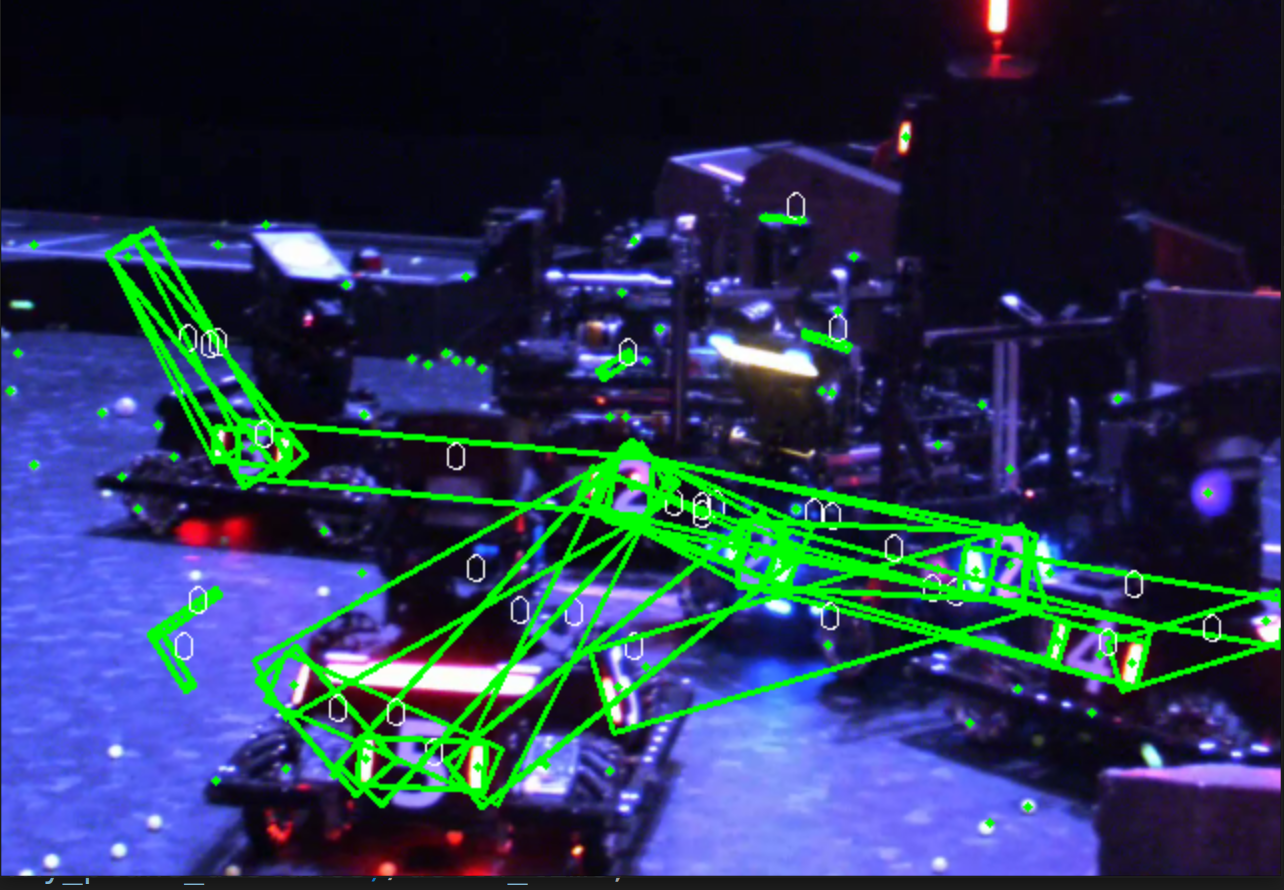
\includegraphics[width=.8\textwidth]{detection_first_stage.png} 
    \caption{传统图像处理算法提取多ROI} 
    \label{传统图像处理算法提取多ROI}
\end{figure}





\section{检测算法的深度学习算法设计}
\subsection{大津二值化算法突显数字特征}
为了尽可能的提高算法运行帧率,则必须尽可能的降低曝光时间,比如,如果算法想要达到300fps,
则最大曝光时间不能超过3.4ms,
又因为装甲板中间的数字图案为不发光体,
所以经常会出现因为图像亮度过低造成数字分类器分类失败的情况。
通过分析装甲板的特征,发现数字图案是白色的,
周围背景是黑色的,尽管数字不发光,但是与背景还是可以区分的,
如果将这一小块区域提取出来使用大津二值化算法\cite{1979A}则能够很好的将背景与图案分割。
如下图\ref{ostu}所示。
\begin{figure}[H]
    \centering
    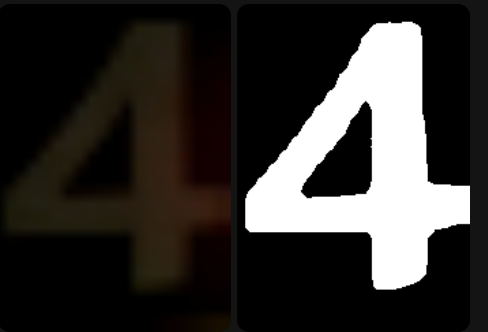
\includegraphics[width=.8\textwidth]{ostu.png} 
    \caption{大津二值化算法效果图,左为原图,右为二值化之后的图像} 
    \label{ostu}
\end{figure}




\subsection{卷积神经网络实现图像分类}

为了防止出现误识别的情况,提取到“装甲板”对应的ROI区域后需要将它们放入分类器去进行分类,此外对于不同的兵种(装甲板对应不同的数字)击打的优先级是不同的,因此对于装甲板类别的判断是非常重要的。\par
目前对于图像分类的方式有许多种,比如基于卷积神经网络方案(如ResNet\cite{2016Deep})和传统机器学习(如SVM)
等。我们的任务是实现装甲板分类,装甲板的特征比较简单但是类别较多,同时还需要具备对于负样本的判断能力,
基于这几个特点选用卷积神经网络实现图像分类任务。
\begin{figure}[H]
    \centering
    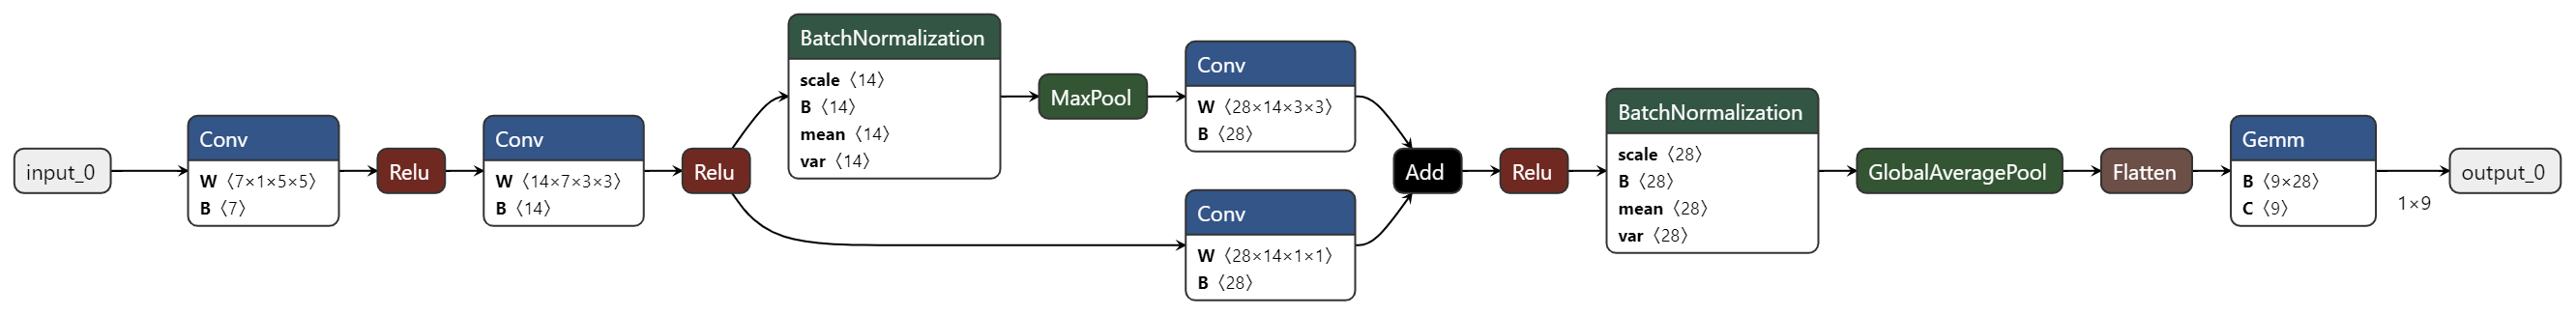
\includegraphics[width=\textwidth]{classify_network_structure.png} 
    \caption{分类器网络结构} 
    \label{分类器网络结构}
\end{figure}
全连接的神经网络虽然形式简单同时也能获得一个较高的准确度,
但是全连接层巨大的参数量会对运行时间造成很大的影响,因此我们考虑使用全局平均池化去解决参数量大的问题,
可使用全局平均池化虽然减少了参数量却丢失了许多信息,测试发现模型收敛后无法达到一个较高的准确度。
对于此问题所采用的解决方案是在两层卷积层之后引入一个残差块,将前两层卷积所提取到的特征信息与第三层卷积层的计算结果融合起来,
然后再去使用全局平均池化,经过测试发现最终它所能达到的准确超过全连接神经网络。网络结构如图\ref{分类器网络结构}所示。


下图\ref{分类器测试结果}展示训练后的神经网络在面对新数据时的表现。可以看到神经网络分类器对于模糊、有噪声干扰、形状不一的图片都有很好的表现。
\begin{figure}[H]
    \centering
    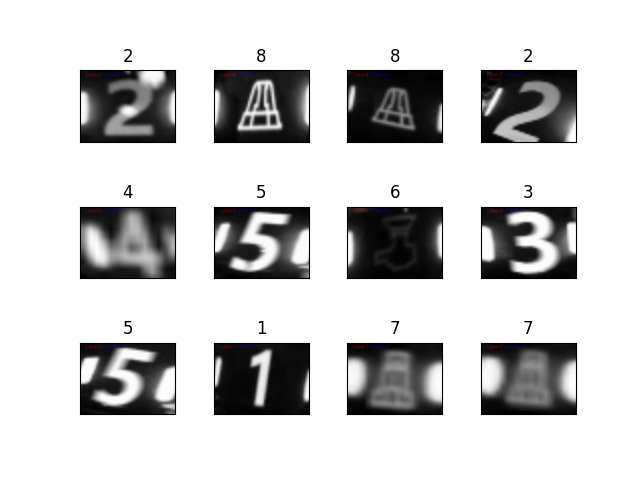
\includegraphics[width=.8\textwidth]{classify_demo.png} 
    \caption{分类器测试结果} 
    \label{分类器测试结果}
\end{figure}

下图\ref{识别算法最终效果展示}展示经过神经网络分类器判别之后得到的装甲板。可以看到经过神经分类器后,一些误识别的区域排除,只留下存在装甲板的区域。
\begin{figure}[H]
    \centering
    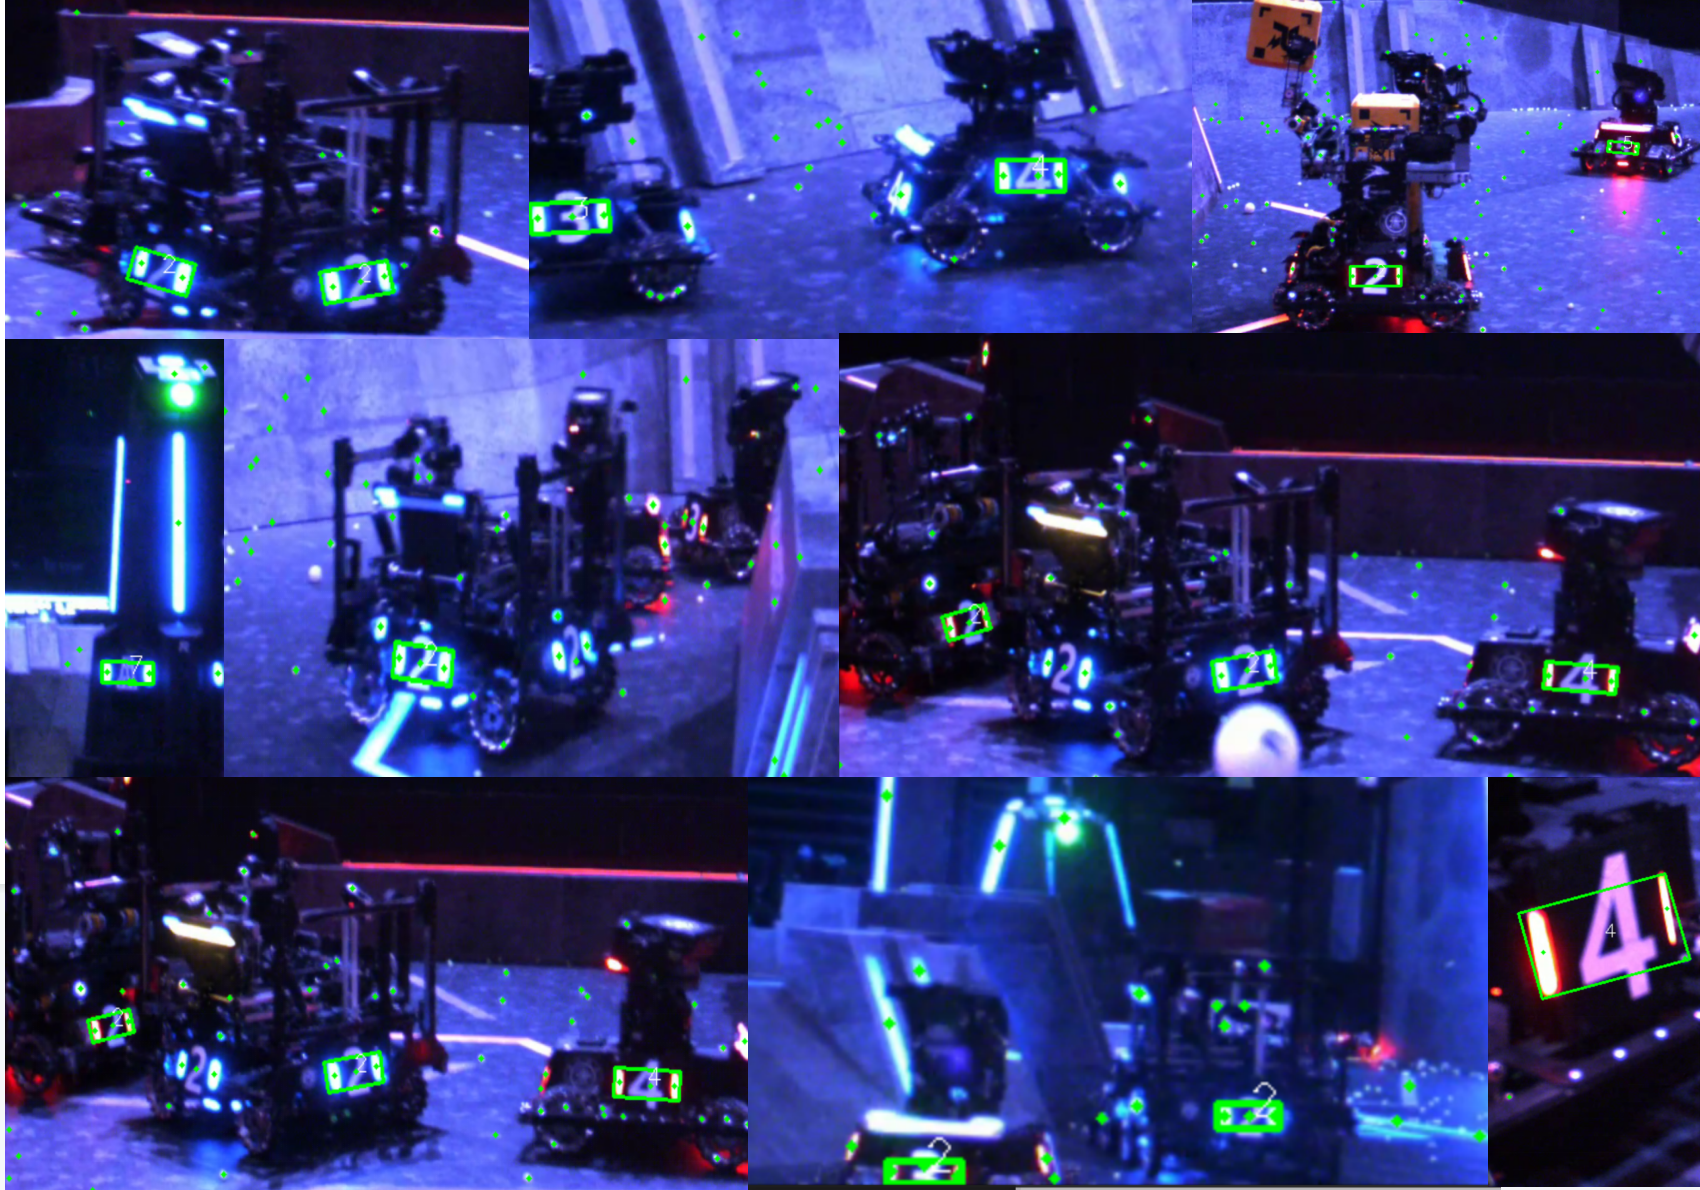
\includegraphics[width=.8\textwidth]{detection_final_result.png} 
    \caption{识别算法最终效果展示,识别到的装甲板被绿色框框出} 
    \label{识别算法最终效果展示}
\end{figure}

\section{本章小结}
将传统数字图像处理与深度学习等技术结合实现装甲板目标的检测。将算法部署在NVIDIA TX2 上,运行平均帧率150fps+,召回率98\%,正确率99\%。检测算法性能满足系统要求。







\chapter[运动预测算法设计]{运动预测算法设计}[Harbin Institute of Technology Postgraduate Dissertation Writing Specifications]


\section{引言}[Content specification]

运动预测本质上是对运动物体的建模,比如,通过观测得到当前物体的位置,
并结合历史观测数据(位置、时间戳等)能够计算出物体的运动信息(如速度、加速度等),
从而能够预测未来在$t$时刻物体的位置,以在一维$x$方向匀速运动的物体为例: 
\begin{gather}
    x(t) = x_0 + v_x*t
\end{gather}

对运动物体的建模即为假定一个运动模型,通过历史数据拟合参数。
比如,匀速运动模型为通过一堆带着时间信息的坐标点去拟合速度。




\section{运动模型的坐标系选择}[Content specification]

通过PnP算法或者是其他算法解算的目标位置(实际上得到的是位置和姿态,
但是运动预测不需要目标的姿态,因此下文只考虑目标的位置)的坐标系是相机坐标系,但是,
云台运动时相机坐标系的位姿也会有变化,观测的相对于大地静止的目标也会发生变化,这样不利于建立运动模型。所以,
需要将目标的位置坐标转换到惯性坐标系下,这样目标点的位置不随着云台运动而运动,从而可以建立准确的运动学模型。\par
由于设备采用的是单目相机,得到某点的信息只有其在$x$和$y$方向的像素坐标信息,
其实得到是目标相对于相机坐标系的$yaw$和$pitch$轴角度信息,
即,相机成像的物理模型使得在观测物体的位置时选择的坐标系为球坐标系。
至于深度信息,即球半径,单目相机在没有先验知识的情况下是无法结算出的。
然而装甲板的实际尺寸大小是已知的(先验),由透镜成像的物理模型(图\ref{透镜成像模型})可得:\par
\begin{gather}
    d = \frac{fh}{y} 
\end{gather}

\begin{figure}[H]
    \centering
    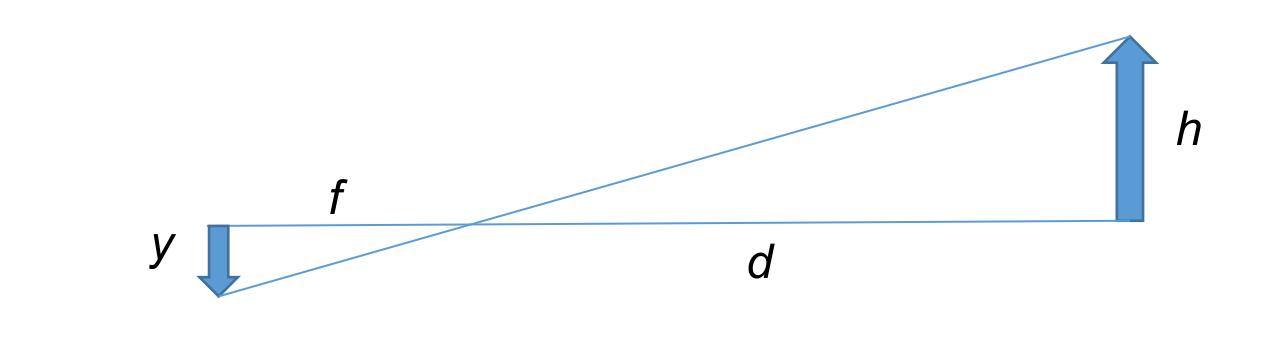
\includegraphics[width=.8\textwidth]{camera_model.png} 
    \caption{透镜成像模型}
    \label{透镜成像模型} 
\end{figure}    
这样,通过计算灯条的像素高度、事先标定好的相机内参中的$f_y$和先验装甲版实际高度就可以计算出目标相对于相机的实际距离。
注意,上面的$y$的单位不是像素,而是$mm$、$m$这样的单位,
而实际从图像上读的是像素值,因此实际的计算公式如下:
\begin{gather}
    d=\frac{fh}{y_{像素}}=\frac{fh}{y*dy}=\frac{f_yh}{y}
\end{gather}
这样,就得到了物体在相机坐标系下的位置描述$(yaw,pitch, distance)$。
当然,可以把它再转换到笛卡尔坐标系$(x,y,z)$。不过需要注意的是,
转换之后的$x,y,z$之间存在耦合关系(例如:x、y都与distancce有关,当distance发生改变时,x、y同时都会改变);
但是$yaw,pitch,distance$之间则相互独立。\par

从计算深度距离$distance$的公式可以看出最大的不确定的因素就是顶点像素的位置,
提取像素点不可能完全的准确。采用图像二值化的方式,提取的轮廓边缘的像素值一定是在阈值附近的,
有时高于阈值,有时低于阈值,影响就是结算出来的距离一直在波动;且随着距离的增加,构成灯条的像素点数减少,像素点的波动对于测距影响增大,影响就是距离越远,测距误差越大。
因为上述所说的噪声不可避免,所以采用卡尔曼滤波器得到距离的最优估计值。\par

\section{运动模型选择}[Content specification]
要使用卡尔曼滤波器,我们首先需要确定运动模型。对于运动模型,首先需要明确的是运动模型实际上是无法用数学公式描述的,
即使能够用数学公式描述对于而言也是不可知的。 所以只能假设它是匀速运动模型或者是匀加速运动模型或是其他运动模型。
对于RoboMaster比赛来说,匀速运动模型能够应对大多数场合。然而,机器人加减速频繁,那么选择匀加速模型是不是更准确呢? 
经过测试发现,引入加速度后,从原先只需要拟合一个参数变成了拟合两个参数,容易造成拟合结果的不准确。且容易产生过拟合现象。
如下图所示,高阶模型固然对已有的点拟合的准确,但从图中\ref{过拟合现象}明显可以看出如果新加一个点,必然与拟合的曲线相差甚大。
\begin{figure}[H]
    \centering
    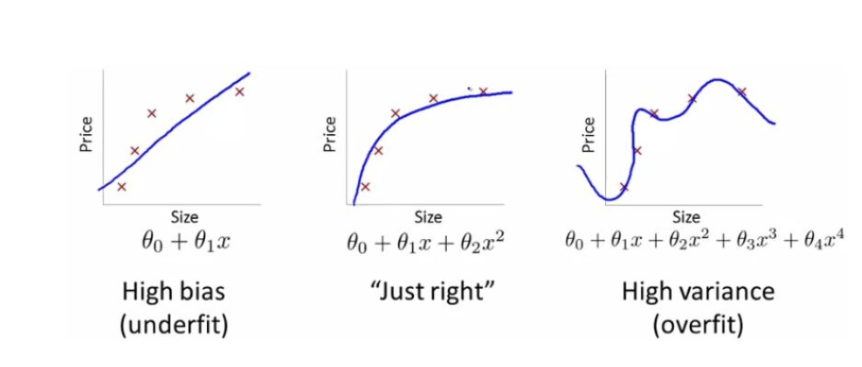
\includegraphics[width=.8\textwidth]{overfit_demo.png} 
    \caption{过拟合现象} 
    \label{过拟合现象} 
\end{figure} 

综上所述,建立的运动模型为$yaw$方向匀速运动,深度方向匀速运动。

\section{基于卡尔曼滤波器建立目标运动模型}[Content specification]

使用卡尔曼滤波器建立物体运动模型过程如下:
将PnP算法解算出目标在相机坐标系 ($c$系)的坐标投影到球坐标系上:
\begin{equation} \boldsymbol p_c=\left[\begin{array}{c} yaw_c\\ pitch_c \\ distance_c \end{array}\right] \end{equation}
\par 
通过机械测量得到相机与云台旋转中心的相对位置,则目标在云台坐标系 ($g$ 系) 的坐标可由 $r_c$经过旋转平移后得到:
\begin{equation} \boldsymbol p_g=\left[\begin{array}{c} yaw_g\\ pitch_g\\ distance_g \end{array}\right] =\boldsymbol C_{c}^{g}\boldsymbol p_c + \boldsymbol t_{c}^{g} \end{equation}
\par 
然后根据陀螺仪数据将云台系坐标转换成惯性系坐标(即对于一个固定目标,即使云台动,观测坐标也不会变化):


\begin{equation} \boldsymbol p_i=\left[\begin{array}{c} yaw_i\\ pitch_i\\ distance_i \end{array}\right] =\boldsymbol C_{g}^{i}\boldsymbol p_g \end{equation}

\par
采用匀速模型描述目标在惯性系的运动,以下为离散形式:
\begin{equation} \boldsymbol x_{k+1} =\left[\begin{array}{cc} {1} & \Delta t  \\ 0 & {1}  \end{array}\right]\boldsymbol x_{k} + \left[\begin{array}{c} {\frac{1}{2}\Delta t^2} \\ {\Delta t}  \end{array}\right]w_k \end{equation}



利用匀速模型设计卡尔曼滤波器以估计目标在惯性系的位置与速度,
设状态变量为:\begin{equation} \boldsymbol x =\left[\begin{array}{c} yaw_i\\ \dot {yaw_i}\\ pitch_i\\ \dot {pitch_i} \\ distance_i\\ \dot {distance_i} \end{array}\right] \end{equation}
\par
过程模型为:\begin{equation} \boldsymbol  x_{k+1} = \boldsymbol F_k\boldsymbol  x_k + \boldsymbol{\Gamma}_{k}\boldsymbol {w}_{k}, \quad \boldsymbol {w}_{k} \sim N\left(\boldsymbol 0_{3 \times 1}, \boldsymbol Q_k \right) \end{equation}

其中: 
\begin{equation} F_k =\left[\begin{array}{cccccc} 1 &  \Delta t & 0 &0&0&0\\ 0 &  1 & 0 &0&0&0\\ 0 & 0 & 1&  \Delta t & 0 &0\\ 0&0&   0&1 &0 &0\\ 0 &0& 0 &0& 1 &\Delta t \\ 0 &0& 0 & 0 &0 &1 \end{array}\right] \end{equation}
\begin{equation} A =\left[\begin{array}{cccccc} 1 &  \Delta t & 0 &0&0&0\\ 0 &  1 & 0 &0&0&0\\ 0 & 0 & 1&  \Delta t & 0 &0\\ 0&0&   0&1 &0 &0\\ 0 &0& 0 &0& 1 &\Delta t \\ 0 &0& 0 & 0 &0 &1 \end{array}\right] \end{equation}

过程噪声方差阵$Q_k$:
\begin{equation} \boldsymbol Q_k =\left[\begin{array}{ccc} \sigma_{yaw}^2 &  0 & 0 \\ 0 &  \sigma_{pitch}^2 & 0 \\ 0 & 0 & \sigma_{distance}^2 \end{array}\right] \end{equation}
\par
其中 $\sigma_{yaw}^2$,$\sigma_{pitch}^2$,$\sigma_{distance}^2$分别$yaw$,$pitch$,$distance$三轴过程噪声方差。
\par


观测模型如下:\begin{equation} \boldsymbol  z_{k} = \boldsymbol H_k\boldsymbol x_k + \boldsymbol {v}_{k} \end{equation}
\par
采用目标惯性系坐标作为量测向量,\begin{equation} p_i = [yaw_i,pitch_i,distance_i]^T \end{equation} 
\par
则:
\begin{equation} \begin{aligned} \boldsymbol H_k &=  \left[\begin{array}{cccccc} 1 & 0 &0 &0 &  0 &0   \\ 0 &0 &1 &0 &0 &0 \\ 0 &0 &0 &0 &1 &0  \end{array}\right],\boldsymbol {v}_{k} \sim N\left(\boldsymbol 0_{3 \times 1}, \boldsymbol {R}_k\right) \end{aligned} \end{equation}
% \\\begin{equation} \begin{aligned} \boldsymbol H_k &=  \left[\begin{array}{cccccc} 1 & 0 &0 &0 &  0 &0   \\ 0 &0 &1 &0 &0 &0 \\ 0 &0 &0 &0 &1 &0  \end{array}\right],\boldsymbol {v}_{k} \sim N\left(\boldsymbol 0_{3 \times 1}, \boldsymbol {R}_k\right) \end{aligned} \end{equation}\\  
% \par
% 根据图\ref{相机模型}相机模型
% \begin{figure}[H]
%     \centering
%     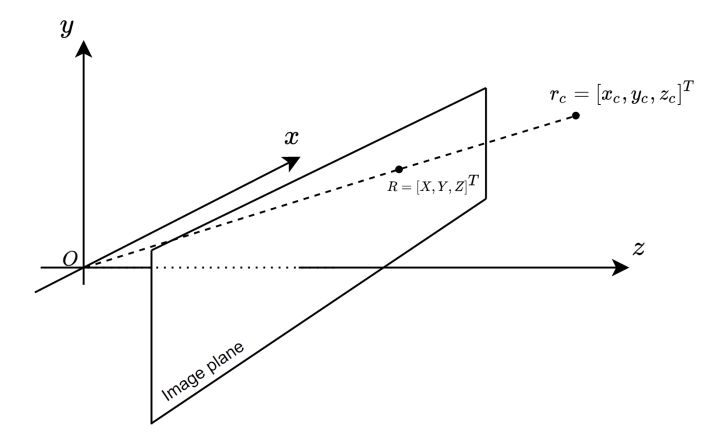
\includegraphics[width=.8\textwidth]{camera_model.jpg} 
%     \caption{相机模型} 
%     \label{相机模型} 
% \end{figure} 
\par

% \section{射频切换设计}[Content specification]
% 尽管射频与运动预测好像没有直接关系,但是射频切换确实依赖于运动预测的。
% 在RoboMaster赛场上,如何把握发弹时机是非常关键的一环。
% 对于敌方车辆在静止状态和匀速运动状态时切换到高射频模式集火攻击非常关键,
% 然而这种情况在一些场景下转瞬即时,
% 如果依赖于操作手手动切换射频往往容易错过时机,因此,选择通过视觉算法作出是否切换长高射频模式。\par

% 对于预测击打,即当敌方车辆处于非陀螺状态时,我们通过判断此时预测器预测质量的好坏来判断是否切换射频。
% 具体来说,射频默认在低射频模式,在当前图像结算出目标的世界坐标后,然后计算子弹飞行时间,
% 根据子弹飞行时间到退到历史预测器,根据历史预测器的状态对当前帧进行预测,并将预测点反投影到图像上,
% 如果反投影点在识别的装甲板矩形框之内,则认为此时预测器质量高,可以切换成高射频模式,
% 电控那边再通过判断此时云台的控制精度是否达到视觉要求的控制精度,满足条件后即可开火。
% 为了防止一些数据跳动,爆发发弹动作进入和退出都需要状态值累积到一定程度,因此设计滞回比较器,使得进入爆发发弹更加容易,退出爆发发弹更加困难。

% 然而,上述使用历史预测器来衡量当前预测器的好坏使得判断产生滞后。
% 即:子弹虚拟飞行时间太长,导致系统滞后明显。
% 那如果我选择使用临近的预测器呢?由于两个预测器相隔时间太近,导致子弹虚拟飞行时间太短,
% 即使预测器的速度信息不准确,但是由于乘以一个时间小量导致总体预测位置偏出不大,即重投影点不具有太高的可信度。
% 因此应该选择一个阈值,比如0.5s。如果通过当前目标计算的子弹飞行时间高于阈值,
% 则选择0.5s之前时刻的历史预测器计算重投影点,低于该阈值则依然采用子弹飞行时间倒推的历史预测器。




\section{运动预测效果分析}[Content specification]

至此,卡尔曼滤波器中所有输入均已确定。在实际测试过程中认知到影响运动预测效果的几个方面:
\begin{enumerate}[itemsep=2pt,topsep=0pt,parsep=0pt]
    \item 识别效果,主要包括正确识别的帧率、灯条角点回归的准确性。
    \item 运动模型建立的准确性。例如:如果物体是加速运动,那么按照匀速运动模型对物体建模就会有偏差。
    \item 噪声设置的准确性。这个影响非常的关键。卡尔曼滤波器的观测噪声和过程噪声都是需要我们手动设置的,然而这些参数是很难通过测量得到的,
    只能够采用手动调参的方式解决。观测噪声相对于测量噪声过大,会导致系统更加依赖预测值,系统跟随性能好,但是面对噪声大的数据容易不稳定,产生震荡;
    观测噪声相对于测量噪声过小,会导致系统更加依赖观测值,系统产生滞后。我得到的调参经验是,先去找一个极小值和极大值,
    然后设置参数为他们的中间值看表现效果,如表现效果更接近极小值,则更新极小值为中间值,反之则更新极大值为中间值。
    \item 目标距离。使用历史信息拟合的速度$v_x$来对未来做预测,但是前提是速度是不变的,
    否则无法利用过去的速度预测未来的位置,在预测时间$t$内,物体的运动速度是可变的,
    积分得到的位移变化量就不是$v_x*t$。然而考虑到物体惯性属性,
    在短时间内速度不会产生较大的突变,实际的位移量与计算的位移量相差不大,那还是可以击中物体的(可以理解为线性近似的误差越小)。
    \item 子弹速度。与目标距离的影响原因一致。子弹速度越大,飞行时间越短,线性近似的误差越小,命中率越高,反之命中率越低。

\end{enumerate}

\section{本章小结}[Content specification]

通过分析相机的观测模型在惯性系下建立物体的匀速运动模型,
将运动模型嵌入到卡尔曼滤波器中,且同时达到平滑数据的效果。





\chapter[追踪算法设计]{追踪算法设计}[Harbin Institute of Technology Postgraduate Dissertation Writing Specifications]

\section{引言}[Content specification]
由于画面中可能存在多块装甲板,若要对装甲板建立运动模型必须明确当前装甲板与历史装甲板的
匹配关系,追踪算法的设计目的就在于此。
在目标追踪算法的设计中,高效、准确是核心考虑因素。
尽管基于深度学习的方法在追踪任务中能够获得非常高的准确率,
但其对计算资源的消耗也是不可忽视的。
\par
因此,本文提出了一种算法设计思路,不依赖于深度学习技术。
该算法为每块装甲板单独建立运动模型,利用模型对当前时刻进行位置预测,
并基于类贪心算法
并通过一一配对来实现目标追踪。

\section{追踪算法设计}[Content specification]

算法设计思路为:为每块装甲板单独建立运动模型,每块有运动模型的装甲板利用运动模型对当前时刻进行位置预测,然后与观测到的装甲板进行一一配对,若距离小于阈值且观测装甲板的数字与携带运动模型对应装甲板的数字一致,
则认为两者同属一块装甲板,利用当前装甲板信息更新运动模型,从而实现追踪效果。
为了实现追踪效果的鲁棒性,允许装甲板的运动模型在短时间不更新,从而起到在受遮挡的情况下依然保留运动模型,待装甲板离开遮挡后不必重新计算运动模型;但是较长时间不更新则认为目标已经不在视野范围内。
\par

另外追踪层级有两层,第一级为追踪同一块装甲板,若追踪同一块装甲板失败,则退而求其次,追踪同一辆车。
因为存在识别算法不稳定或者是装甲板被遮挡等因素造成的识别丢帧现象,
所以在追踪模式下(包括追踪同一块装甲板模式和追踪同一辆车模式)允许一定数量的丢帧。
基本思路为:设置三个模式:搜索装甲板模式,追踪装甲板模式,以及追踪车辆模式,
初始状态标记设为搜索装甲板模式。

\begin{itemize}[itemindent=2em]
\item 在搜索装甲板模式下,如果搜索到装甲板则将标记位设置为追踪装甲板模式,且将该装甲板设置为追踪目标。
\item 在搜索装甲板模式下,如果未搜索到装甲板则直接返回。
\item 在追踪装甲板模式下,在装甲板丢帧次数低于追踪通装甲板丢帧阈值的情况下识别到追踪目标,则将装甲板丢帧次数清零,且更新追踪目标为当前检测到的装甲板。
\item 在追踪装甲板模式下,在装甲板丢帧次数低于追踪通装甲板丢帧阈值的情况下未识别到追踪目标,则将次数增加1。
\item 在追踪装甲板模式下,在若装甲板丢帧次数高于追踪通装甲板丢帧阈值的情况下则将标记为设置为追踪车辆模式,且装甲板丢帧次数清零。
\item 在追踪车辆模式下,在车辆丢帧次数低于追踪车辆丢帧阈值的情况下识别到同一辆车的其他装甲板,则将车辆丢帧次数清零,且更新追踪目标为当前检测到的装甲板,且将标记为设置为追踪装甲板模式。
\item 在追踪车辆模式下,在车辆丢帧次数低于追踪车辆丢帧阈值的情况下未识别到同一辆车的其他装甲板,则将车辆丢帧次数加1。
\item 在追踪车辆模式下,在车辆丢帧次数高于追踪车辆丢帧阈值的情况下,将标记为设置为搜索装甲板模式,装甲板丢帧次数清零,车辆丢帧次数清零。
\end{itemize}

追踪逻辑如图\ref{追踪算法逻辑图}所示:

\begin{figure}[H]
    \centering
    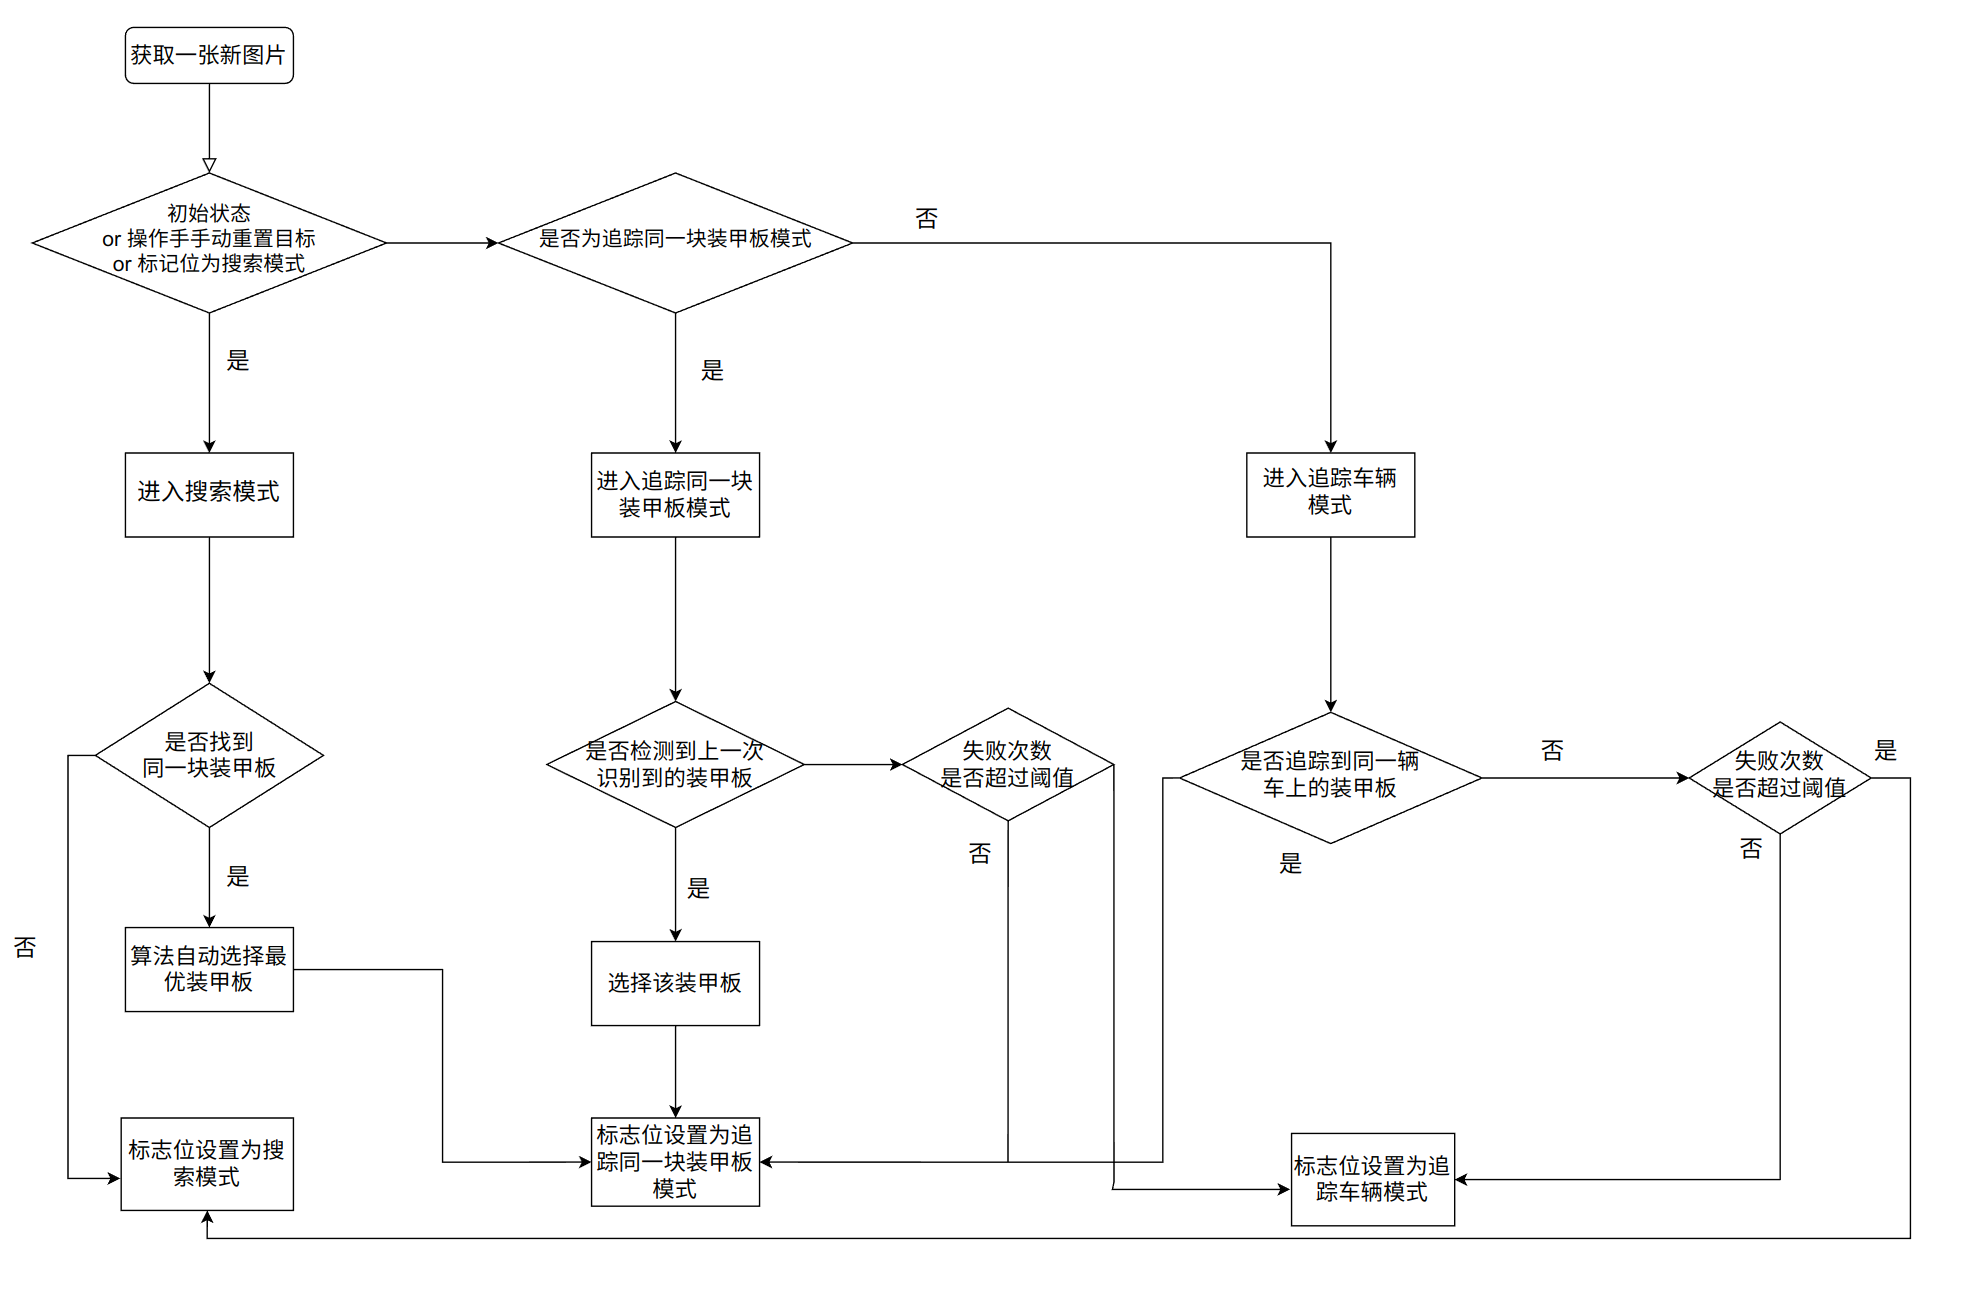
\includegraphics[width=.99\textwidth]{track_chart.png} 
    \caption{追踪算法逻辑图} 
    \label{追踪算法逻辑图} 
\end{figure} 

\par


\section{本章小结}[Content specification]


本章基于运动模型的设计了一种追踪算法,目的是为了建立装甲板与历史装甲板之间的匹配关系。
该算法为每个装甲板建立单独的运动模型,
然后将当前时刻的位置预测与观测到的装甲板进行一一配对,
通过更新运动模型来实现追踪效果。该算法设计了两个追踪层级,
第一级是追踪同一块装甲板,第二级是退而求其次,追踪同一辆车的不同装甲板。
为了提高算法的鲁棒性,该算法允许运动模型在短时间内不更新,
从而在装甲板受遮挡时保留运动模型,但长时间不更新则认为目标已不在视野范围内,效果如图ref{kalman_gpt}所示。

\begin{figure}[H]
    \centering
    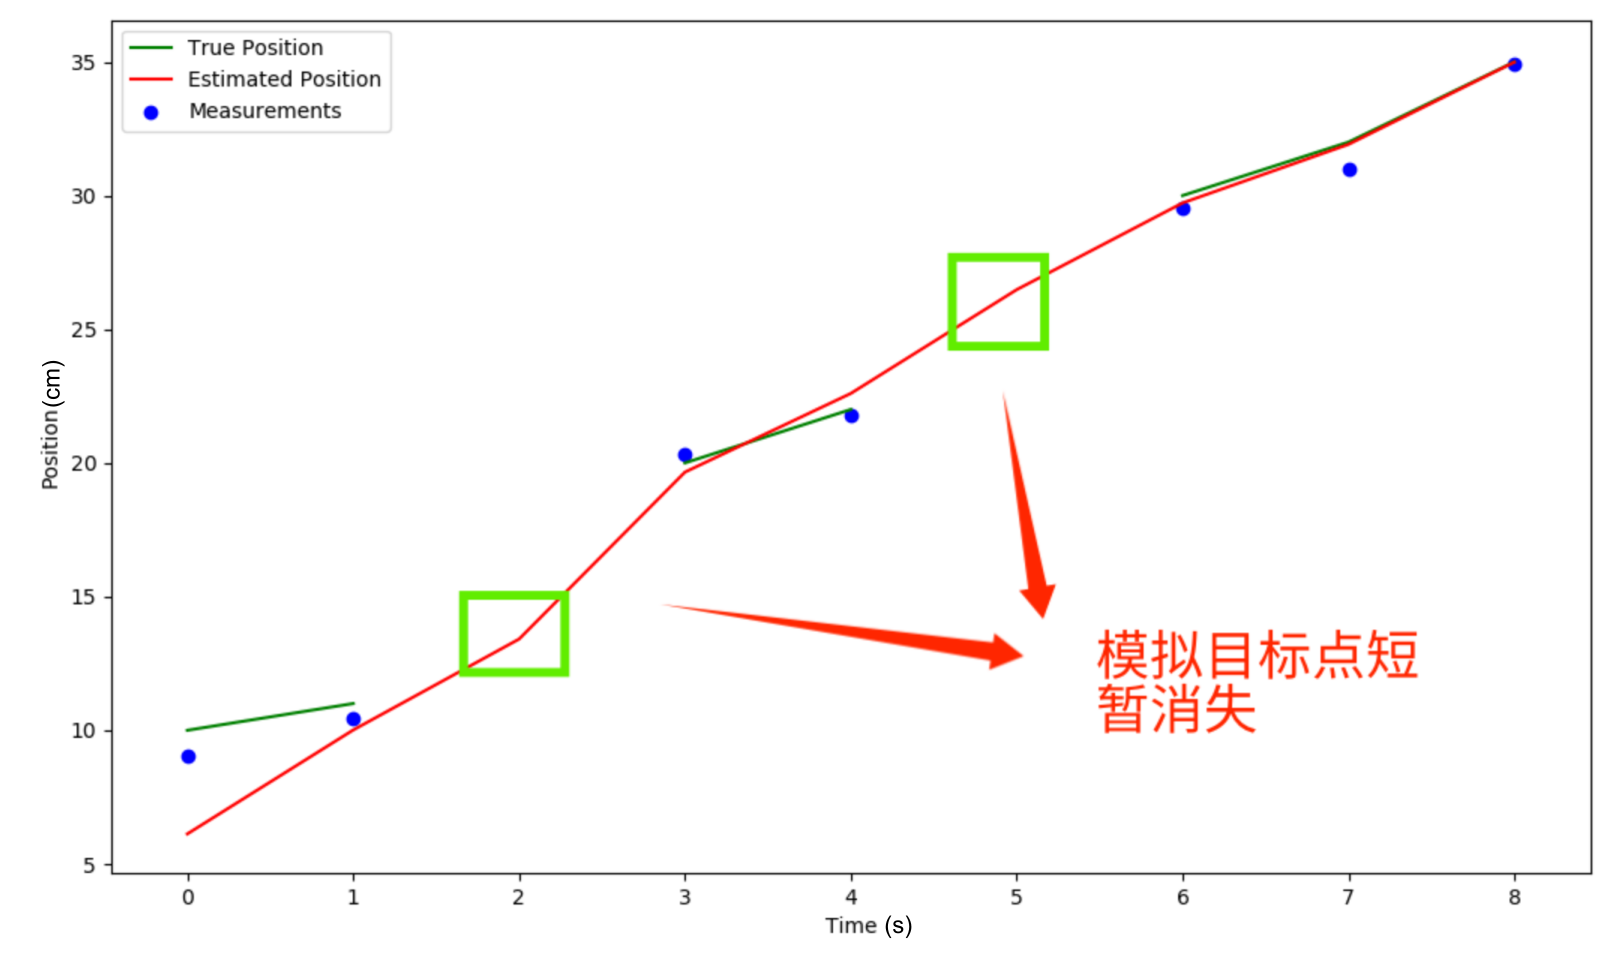
\includegraphics[width=.8\textwidth]{kalman_gpt.png} 
    \caption{目标追踪鲁棒性测试} 
    \label{kalman_gpt} 
\end{figure} 

\par
本章为算法设计了三种模式:搜索装甲板模式、
追踪装甲板模式和追踪车辆模式,通过标记位的设置来实现状态的转换。
提高算法的鲁棒性。该算法没有使用深度学习方法,注重算法的效率和准确性。
实现效果如图\ref{pred_merge}所示,目标从左向右移动,云台也追踪着目标从左向右移动。

\begin{figure}[H]
    \centering
    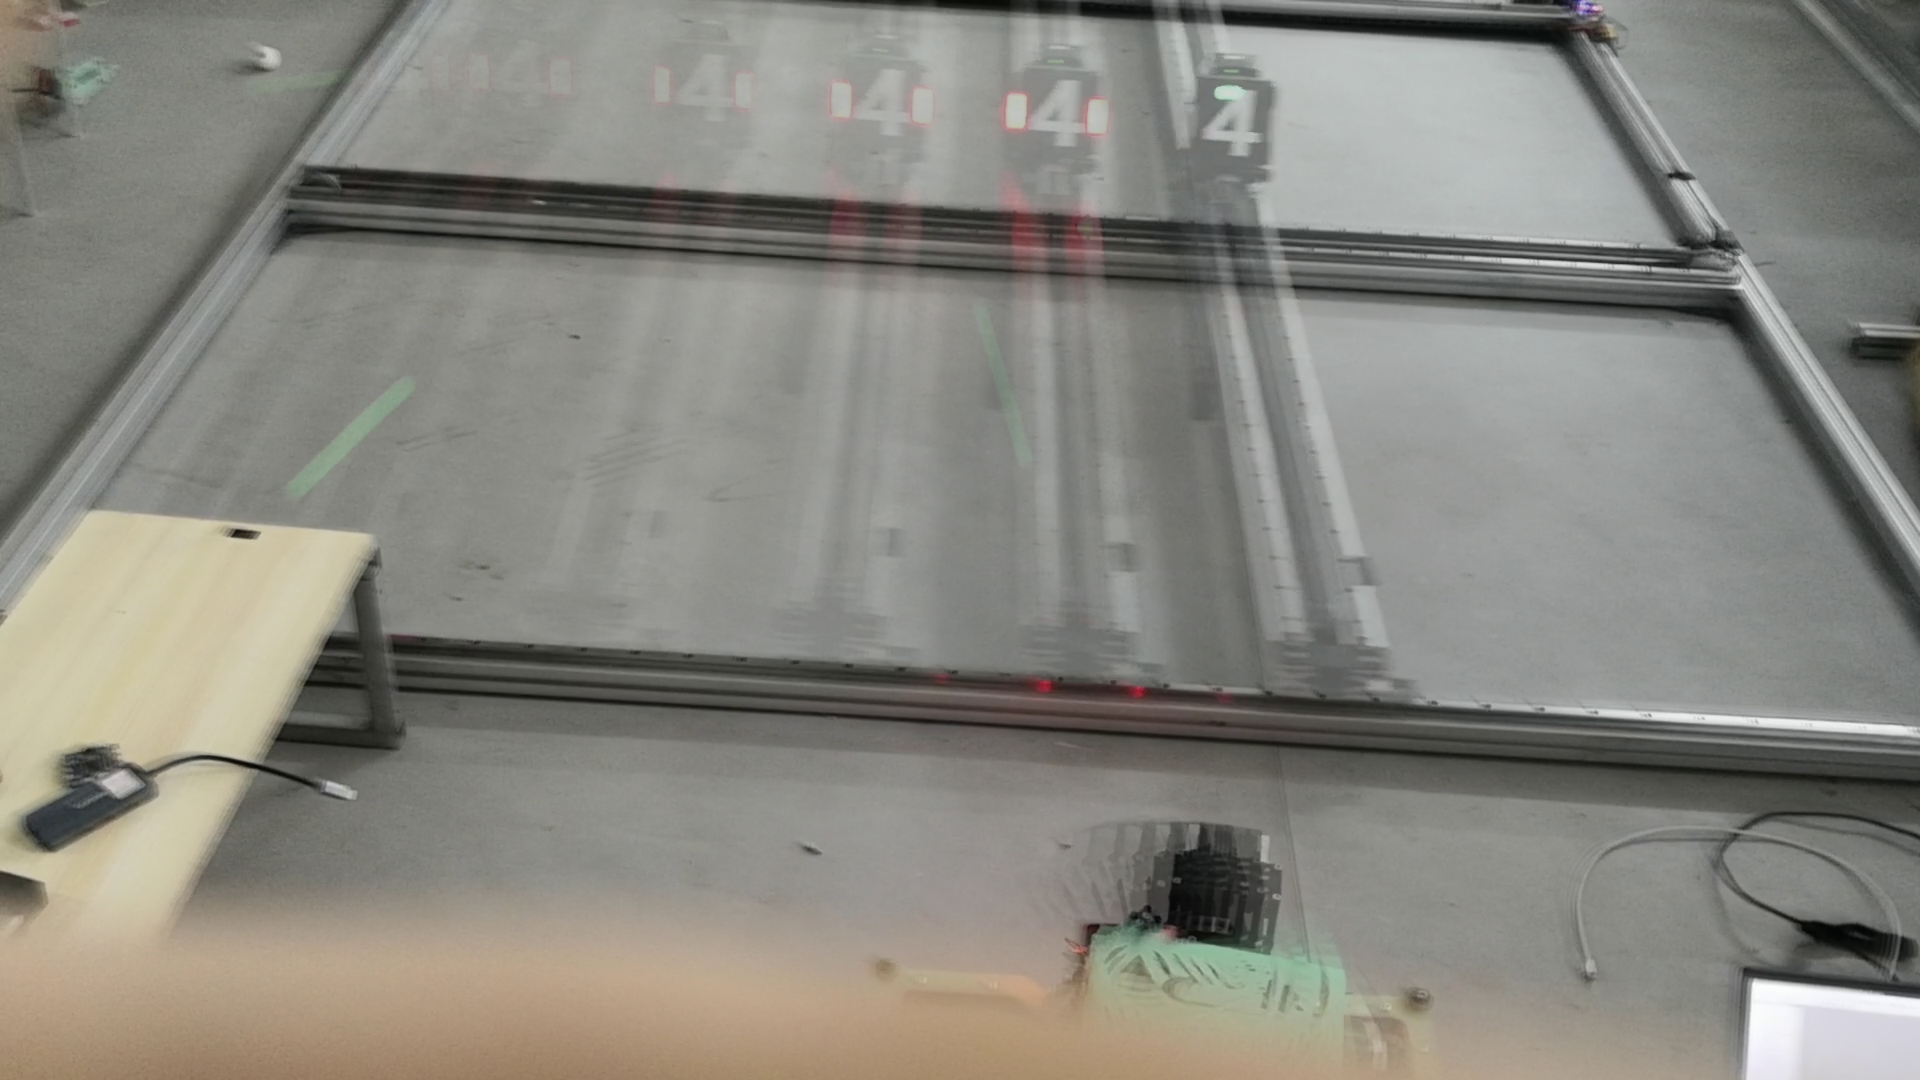
\includegraphics[width=.8\textwidth]{pred_merge.png} 
    \caption{目标追踪效果展示} 
    \label{pred_merge} 
\end{figure} 


\chapter[旋转目标追踪预测]{旋转目标追踪预测}[Harbin Institute of Technology Postgraduate Dissertation Writing Specifications]

\section{引言}[Content specification]
车辆旋转会带动四周的装甲板旋转。
我们将旋转运动称之为陀螺运动。将针对于旋转目标追踪预测的算法称之为反陀螺算法。
之所以引入反陀螺算法,是因为在敌方陀螺运动下,
装甲板是圆周运动,具有强烈的非线性,而运动预测只适合线性模型。
且水平速度巨大,反复切换,出现时间短,
出现子弹还没有飞过去装甲板就已经消失的情况,需要设计专门的追踪预测算法。

\section{反陀螺模型建立}[Content specification]

基于在笛卡尔坐标系建立的全车观测模型对于观测精度的要求极高,且在中远距离以上(>4m)表现效果不佳。
于是以我方车辆为原点建立圆柱坐标系,如图ref{反陀螺坐标系}所示。原因有二:一是对于陀螺运动的敌方车辆我们更加关注于装甲板在yaw方向的运动;二是相机观测模型保证了yaw方向的观测精度。
同时,对于变量的数值我们采用相应的滤波算法处理,对于理论上不发生变换的变量我们采用均值滤波算法,对于可能发生变化的变量我们采用一阶滞后滤波算法处理。
\begin{figure}[H]
    \centering
    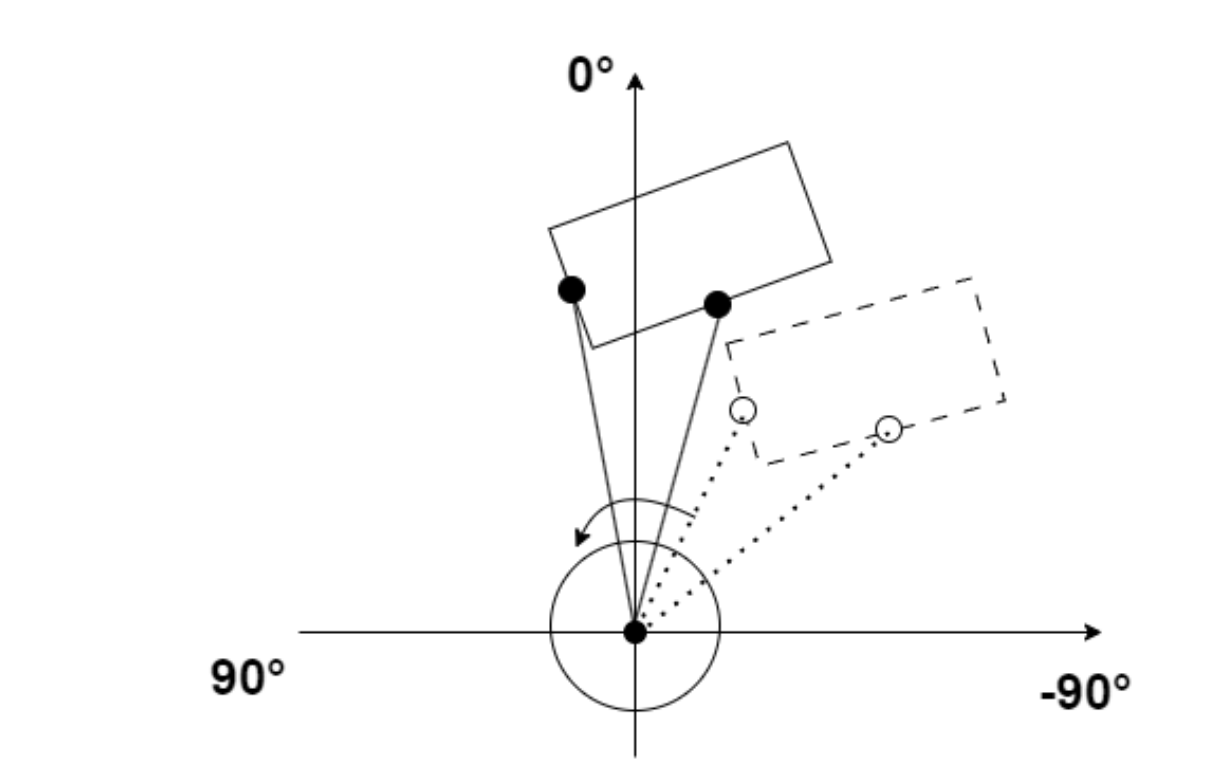
\includegraphics[width=.8\textwidth]{gyro_axis.png} 
    \caption{反陀螺坐标系} 
    \label{反陀螺坐标系}
\end{figure}



\par
在敌方车辆进行陀螺运动时,会发生装甲板切换,在装甲板切换时记录上一次的装甲板和当前装甲板,
记录为小陀螺运动的最左端和最右端。由于车辆四边都有装甲板,则在任意时刻,左右端的中间区域都会有装甲板出现,
即在任意时刻,不考虑云台响应的情况下能够命中目标。


反陀螺模型需要计算以下信息:
\begin{itemize}[itemindent=2em]
    \item 前后和左右两组装甲板的平均高度。采用均值滤波算法。
    \item 整车装甲板的平均高度。采用均值滤波算法。
    \item 陀螺周期$gyro\_period$。一次装甲板切换为0.25个周期,采用一阶滞后滤波算法处理数据,滤波系数0.2。
    \item 陀螺方向。通过角速度判断,且经过积分滤波算法处理。
    \item 最左端和最右端分别对应的$yaw\_left$和$yaw\_right$角度。采用一阶滞后滤波的形式平滑数据,滤波系数0.2。
    \item 陀螺区间$yaw\_section =0.5 \times (yaw\_left + yaw\_right)$。由于参与计算$yaw\_section$的变量已经经过滞后滤波,因此该变量不再滤波。
    \item 装甲板的平均深度信息$d$。采用一阶滞后滤波算法处理,滤波器系数0.5.
\end{itemize}

在得到这些数据后,我们就可以完全描述陀螺运动的车辆。
下图\ref{基于陀螺模型计算的yaw角度与真实yaw角度对比}展示根据陀螺模型计算的装甲板yaw角度与真实角度之差,
其中蓝色的为实时检测到目标的yaw值,红色的为利用前面的数据预测的该时刻的yaw数据。

\begin{figure}[H]
    \centering
    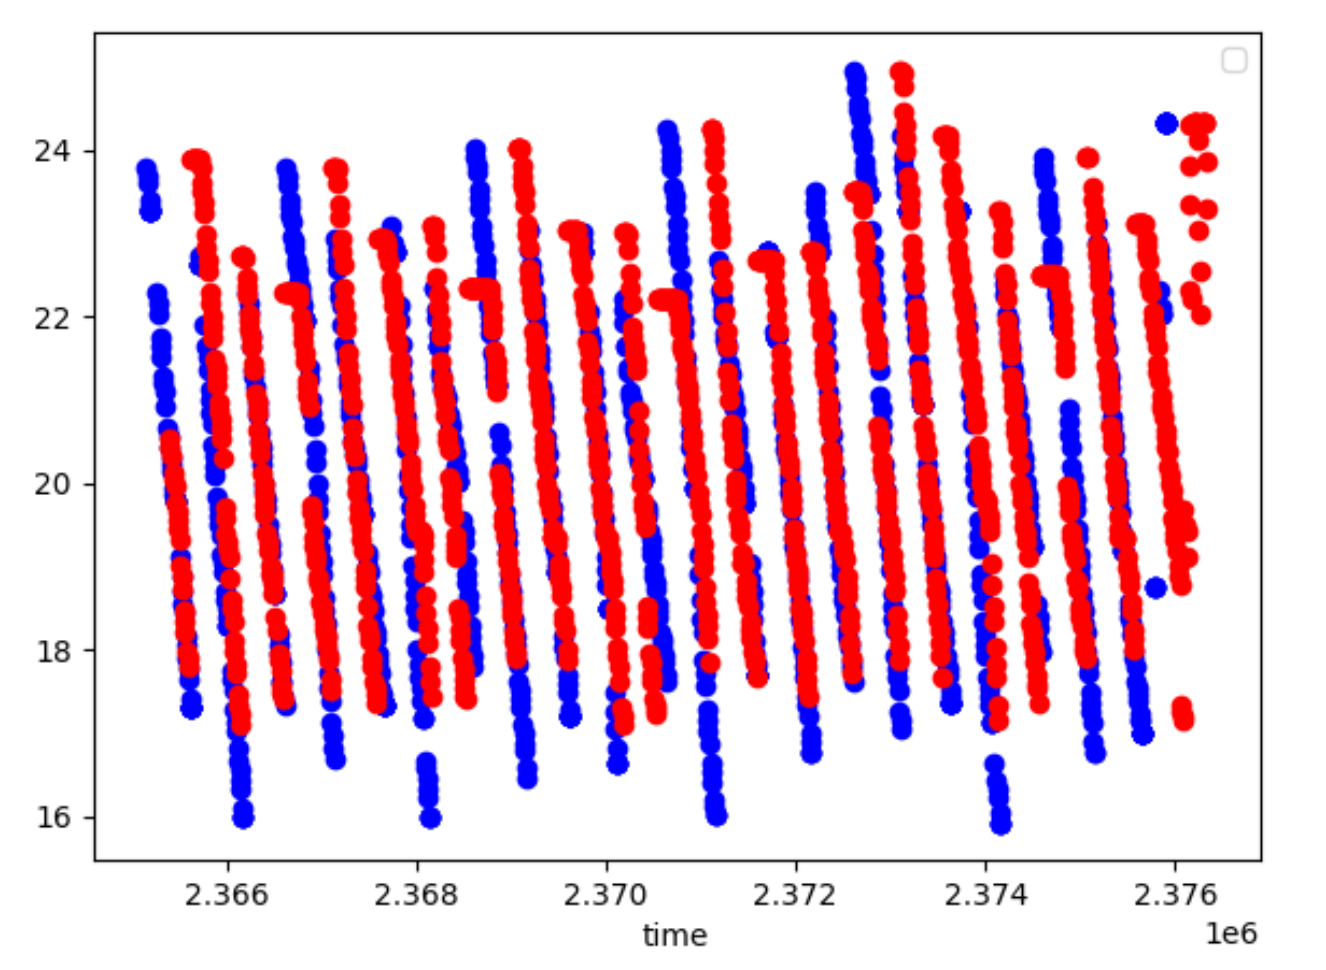
\includegraphics[width=.8\textwidth]{gyro_yaw.png} 
    \caption{反陀螺坐标系} 
    \label{基于陀螺模型计算的yaw角度与真实yaw角度对比}
\end{figure}

\section{云台姿态角求解}[Content specification]


该算法的核心是计算云台yaw和pitch姿态角。计算过程如下:
认为陀螺运动下无论是深度信息的变化(受陀螺运动和平移运动共同影响)还是装甲板高度的变换(受装甲板切换的影响,一般情况下左右和前后两组装甲板的高度不同)
对于子弹飞行时间的影响都是非常小的,即对方在陀螺运动情况下,子弹无论击打到哪个位置的装甲板飞行时间都是相同的。
因此根据上述陀螺模型计算的装甲板的平均深度信息和整车装甲板的平均高度计算子弹飞行时间,
再加入程序延时(当前时刻—上一次装甲板切换时刻),记为时间$t$。
根据时间$t$计算陀螺转了整数$n$个1/4圈,且余数为$m$。




\subsection{Pitch角度求解}[Content specification]
基于$n$计算pitch角度。
\begin{itemize}[itemindent=2em]
    \item 敌方机器人向左转,若$n$是偶数,选择右侧装甲板的高度作为弹道解算的装甲板高度。
    \item 敌方机器人向左转,若$n$是奇数,选择左侧装甲板的高度作为弹道解算的装甲板高度。
    \item 敌方机器人向右转,若$n$是偶数,选择左侧装甲板的高度作为弹道解算的装甲板高度。
    \item 敌方机器人向右转,若$n$是奇数,选择右侧装甲板的高度作为弹道解算的装甲板高度。
\end{itemize}

在得到装甲板高度信息和装甲板平均深度信息$d$后就可以求解pitch轴角度信息。

\subsection{Yaw角度求解}[Content specification]
基于$m$计算yaw角度,计算其相对于最左端或者是最右端(与转动方向有关,如果是往左传,则相对于右端,反之相对于左端)转动的yaw角度。
\begin{lstlisting}
    radio = double(4.0 * time / period)- int(4.0 * time / period);
    delta_yaw = yaw_section * radio;
\end{lstlisting}

我们将陀螺击打过程分为两个部分,云台跟随当前装甲板状态和云台回调迎接下一块装甲板状态。
云台跟随我们认为是无误差的,因为跟随量很小,但是回调量非常大,回调时间不可忽略。
考虑如下情况,对于一块从左向右(陀螺方向)旋转的装甲板,由于云台响应需要时间,
即云台并不能瞬时从最右端回调到最左端,
我们可以选择在放弃击打陀螺区间的后半程,即放弃选择击打最右端,提前将云台回调迎接下一块装甲板;也可以选择
放弃击打陀螺区间的前半程,即放弃选择击打最左端。
在分析识别算法之后发现,由于追踪算法的存在,使得检测的最右端装甲板相对于相机非常倾斜,而此时在左侧装甲板已经出现且相对于相机较为正对。
正对的装甲板不仅投影面积更大,更好击打;而且子弹与装甲板接触的法向速度更大,更不容易被裁判系统漏掉,因此选择放弃击打陀螺的后半程。
我们将选择击打的陀螺区间相对于陀螺整个区间记为r,假设云台最大角速度为$yaw\_speed_{gimbal}$,陀螺观测角速度为$yaw\_speed_{car}$
,则有如下公式:
\begin{gather}
    t  \times (yaw\_speed_{gimbal} + yaw\_speed_{car}) = yaw\_section \\
    r = \frac{t \times yaw\_speed_{gimbal} }{yaw\_section}
\end{gather}
从而求得
\begin{gather}
    r = \frac{yaw\_speed_{gimbal}}{yaw\_speed_{gimbal} + yaw\_speed_{car}}
\end{gather}

最后得到的陀螺区间角度计算公式如下(将该角度加到左端角度或右端角度)即为最终云台设定yaw角度。
\begin{lstlisting}
    radio = double(4.0 * time / period)- int(4.0 * time / period);
    r = yaw_speed_gimbal / (yaw_speed_gimbal + yaw_speed_car);
    if (radio > r) // 超出击打陀螺区间
    {
        radio = 0; // 云台提前回调
    }
    delta_yaw = yaw_section * radio;
\end{lstlisting}

\section{基于反陀螺模型求解发弹时机}[Content specification]
由于云台回调期理论上是打不中目标的,因此这一阶段我们选择不发弹。
即通过判断子弹飞过去的时间对应的装甲板所处区间,
如果区间位于radio以内,则允许发弹,否则不允许发弹。
\begin{lstlisting}
// t1 子弹飞行时间
// t2 程序时延
// t3 发弹延迟
double t = t1 + t2 + t3;
double radio_with_shoot_delay = double(4.0 * t / period) - int(4.0 * t / period);
if (radio_with_shoot_delay < radio)
{
    fire = true;
} else
{
    fire = false;
}
\end{lstlisting}



\section{基于积分滤波器的陀螺方向判断}[Content specification]

算法在每个时刻将当前的yaw\_speed累加到left\_dir\_cnt上,
从而得到一个表示yaw\_speed累积值的left\_dir\_cnt。
在每个时刻根据left\_dir\_cnt的值来判断机器人当前的旋转方向,
如果left\_dir\_cnt超过了一定阈值cnt\_thresh,
就认为机器人在相应的方向上旋转了,
并将left\_dir\_cnt重置为一个较小的值,以避免累积过多的误差。

因此,可以将该算法看作是一种积分滤波算法,
它的作用是平滑yaw\_speed信号,抑制噪声和误差的影响,从而得到更加可靠的旋转方向判断。
具体代码如下:

\begin{lstlisting}
    void AntiGyro::judge_rotate_dir(double yaw_speed, ArmorDir &dir)
    {
        const int cnt_thresh = 5;
        static int left_dir_cnt = 0;
        if (yaw_speed > 0){
            ++left_dir_cnt;
        } else if (yaw_speed < 0)
        {
            --left_dir_cnt;
        } 
        if (left_dir_cnt > cnt_thresh){
            dir = ArmorDir::LEFT;
            left_dir_cnt = 5;
        } else if (left_dir_cnt < -cnt_thresh){    
            dir = ArmorDir::RIGHT;
            left_dir_cnt = -5;
        } else {
            dir = ArmorDir::UNKNOWN;
        }
    }
\end{lstlisting}


\section{本章小结}[Content specification]

通过分析观测量的精度情况和装甲板的运动情况,在惯性系下建立反陀螺模型的圆柱坐标系,
巧妙的避开了三维坐标测量不准的情况。通过装甲板切换频率判断是否进入反陀螺模型,
基于观测的空间量和时间量计算反陀螺模式的所需信息,实现针对敌方车辆以陀螺模式运动的专门击打算法。



\chapter[系统集成功能]{系统集成功能}[Harbin Institute of Technology Postgraduate Dissertation Writing Specifications]

\section{相机选型与基本设置}[Content specification]

\subsection{引言}[Content specification]
相机是计算机视觉中非常重要的一部分,负责获取环境中的图像信息,为后续的图像处理和算法提供输入数据。
因此,在进行计算机视觉项目时,选择适合的相机和合理的设置相机参数设置是非常关键的。
本章根据RoboMaster比赛的赛场光照环境和检测算法要求选择合适的工业相机并给出具体的型号。

\subsection{相机选型策略}[Content specification]
尽量选择高帧率、感光片大的相机,在此基础上选择光圈大的镜头,焦距选择视情况而定。
下面详细阐述:\par

\begin{itemize}[itemindent=2em]
    \item 分辨率:一般分辨率越高,图像质量越好,越有利于识别算法和测距算法。但分辨率越高,图像最大采集帧率越低,
    且检测算法耗时增加,价格也相应越高。因此选择分辨率在30万到100万像素的相机即可。
    \item 帧率:帧率越高,运动图像捕捉能力越好。由于我们需要检测高速移动或者旋转的目标,因此帧率越高越好。
    根据应用场景需要捕捉的运动速度和动态要求,选择适合的帧率,对于RoboMaster比赛场景来说,150fps+的帧率能够满足基本要求。
    \item 传感器尺寸和类型:CMOS和CCD是现代数字图像传感器的两种常见类型。
    CMOS传感器具有低功耗、低噪声、高帧率等优点,且质量更小,所以选择CMOS相机。
    \item CMOS传感器有两种快门方式,卷帘快门和全局快门\cite{huang2023review}。
    全局快门曝光时间更短,但噪声更大;卷帘快门可以达到更高的帧速,但当
    曝光时间较长或物体移动较快时产生果冻效应。
    为了适应RoboMaster比赛场景的需求,选择全局快门的相机。
    \item 工作温度和防护等级:根据应用环境和需求,选择适合的工作温度和防护等级。
    工业相机一般需要在恶劣环境下工作,如高温、灰尘等,所以防护等级要求较高。
    \item 软件支持:算法运行环境为Linux,
    工业相机的软件平台需要支持图像处理和数据分析等功能,
    通常需要与特定的软件开发工具包配合使用,且售后的技术支持和SDK软件包的是否适合二次开发也是选择的考量重点。

\end{itemize}


一张成像清晰、亮度均匀的图片非常有利于后续的图像处理算法,因此如何设置相机参数,以及如何预处理原始图像后都非常重要。
\subsection{相机硬件设置}[Content specification]
拿到相机后,基本设置如下:将光圈拧到最大;调整成像平面与光心的距离,使得5m成像最清晰;涂抹螺丝胶,防止相机在剧烈震动的情况下因螺丝松动而成像不清。之所以将光圈拧到最大,是为了在达到相同图像亮度的情况下获得更短的曝光时间,进而提高相机帧率。
\subsection{相机软件设置}[Content specification]
模拟增益调高,目的:一是在达到相同图像亮度的情况尽可能减少曝光时间从而提高取图帧率,
不过由于增益拉高后图像噪点也会增加,因此需要平衡; 
二是使得发光体在图像中更加明显,从而二值化阈值可以取到非常高,可以防止过曝给灯条的提取造成影响,
因为即使在过曝的情况下,光晕的灰度值与真正的发光体还是有较大的区别,通过高阈值筛选可以很好的提取灯条。

设置相机白平衡参数,使得成像色彩正常,
迈德威视相机的软件工具包提供了自动调节白平衡参数的功能,只需要将相机对准白色物体,
然后点击“白平衡”按钮即可。




\section{主从机时钟对齐}[Content specification]


\subsection{引言}[Content specification]
在工业自动化和嵌入式系统中,上位机和下位机之间的时间同步是非常重要的。通常,下位机的时间通常是由硬件时钟提供的,
而上位机的时间通常是由操作系统提供的。由于硬件时钟和操作系统时钟存在不同步的可能,
因此需要基于通信方法来同步它们的时间,比如网络时间协议(Network Time Protoco, NTP)\cite{sommars2022client}就是一种用于同步计算机时钟的协议。
\par

然而由于下位机目前不支持网络服务,
因此本章参考NTP同步时钟的思路,通过上下位机的控制器局域网(Controller Area Network, CAN)通信实现了双机时钟的统一,
巧妙地解决了网络服务不可达的问题。

\subsection{通信时延测量}[Content specification]
对于一固定的装甲板,晃动云台,则理论上解算的装甲板在惯性系下的坐标是不变的。
然而,由于通信时延、相机成像时间误差、计时精度、陀螺仪数据精度与系统偏差等因素,
不可能精确的获得的图像对应的陀螺仪数据。这里面影响因素最大的就是通信时延,因此通过调节通信时延量,
使得惯性系下的装甲板坐标晃动幅度最后,此时得到的通信时延量被认为是真实的通信时延。
\par
图\ref{delay}展示了在通信时延量在超前、滞后、大致准确时解算的装甲板在惯性下的坐标。
\begin{figure}[H]
    \centering
    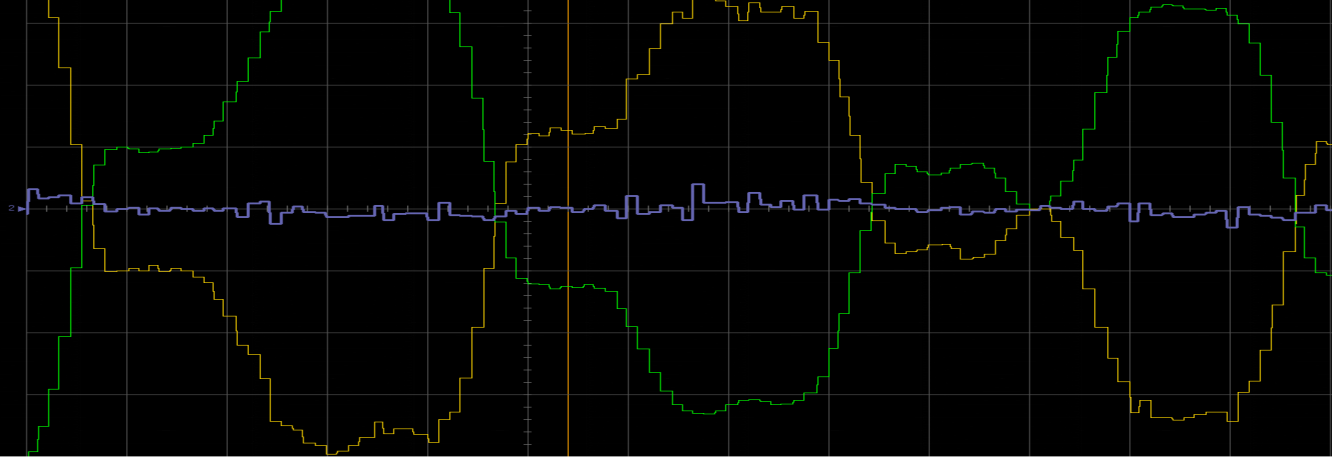
\includegraphics[width=.8\textwidth]{delay.png} 
    \caption{不同通信时延对应的装甲板惯性系下的坐标} 
    \label{delay}
\end{figure}

\subsection{动态时间帧对齐}[Content specification]

基本思想如下:事先通过上述技术手段测量通信时延。然后以下位机的时钟为基准,下位机定频(100$hz$)向上位机发送本机的时钟信息,上位机将计算本机时钟与下位机时钟之差(在考虑通信时延的情况下),
并将数据放入到循环队列中,当需要在上位机获取下位机时钟时刻时,
通过计算循环队列的平均值作为上下位机时钟偏移量加到本机时钟就可以获得下位机的时钟时刻,如图\ref{clock_sync}所示。

\begin{figure}[H]
    \centering
    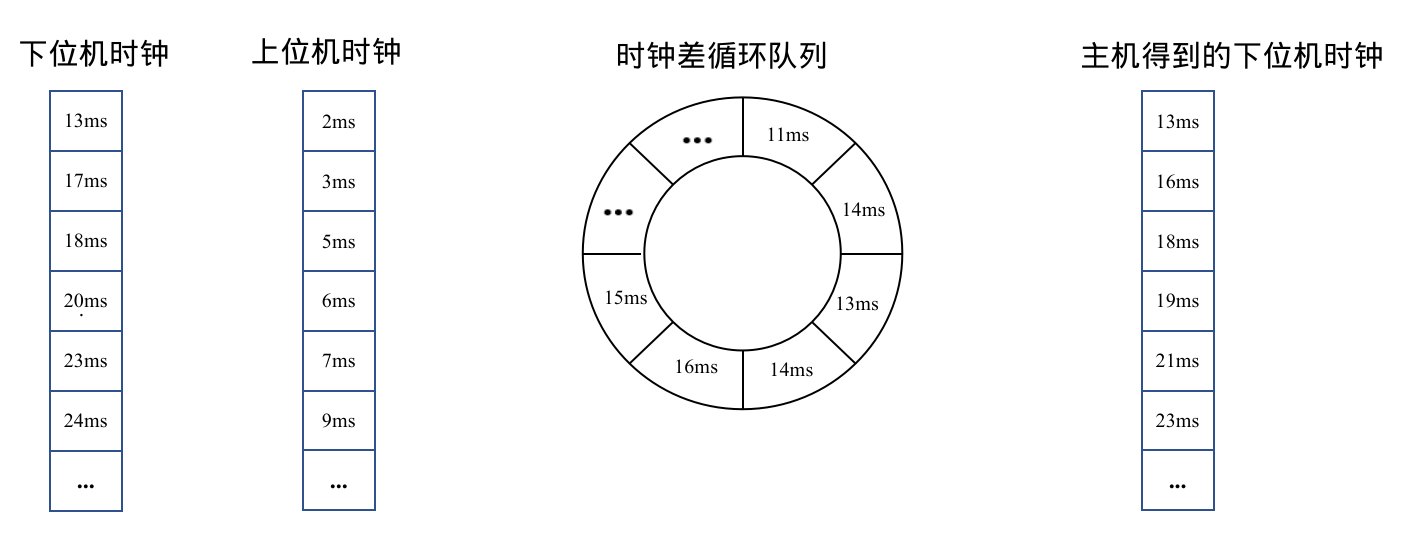
\includegraphics[width=.8\textwidth]{clock_sync.png} 
    \caption{自实现时钟同步} 
    \label{clock_sync}
\end{figure}




\section{受空气阻力的弹道迭代计算}[Content specification]


\subsection{引言}[Content specification]
在现代计算机计算中,迭代计算已经成为了一种非常重要的计算方法,
尤其是在物理学、工程学和计算机科学等领域中。
受空气阻力的影响,
弹道轨迹并不是一个简单的抛物线,
因此迭代计算成为了计算弹道轨迹的重要方法。


\subsection{空气阻力系数求解}[Content specification]
其中因为在$y$⽅向分速度较⼩,可以忽略不计,因此只考虑$x$⽅向的空⽓阻⼒。空气阻力计算见公式(6-1)。
\begin{gather}
    F = kv^2 =  \frac{1}{2} C_dS \rho  v^2
\end{gather}

\par

其中$F$为阻力,$k$为最终空气阻力系数,$\rho$为空气密度,一般取$1.293kg/m^3$,$S$为球截面积,$v$为球体速度,$C_d$为阻力系数,与雷诺数$R_e$有关系,雷诺数计算见公式(6-2)。
\begin{gather}
    R_e = \frac{\rho v D}{\eta}
\end{gather}

其中$R_e$为雷诺数,$\rho$为空气密度,一般取$1.293kg/m^3$,$D$为物体直径,$v$为球体速度,$\eta$为空气粘滞系数,通常取$1.983\times10^{-5}pa\cdot s$。 


\subsection{弹道迭代计算}

我们只考虑水平方向的空气阻力。弹丸的动力学微分方程见公式(6-3)和(6-4),
分别代表在水平方向和竖直方向的动力学方程。其中$m$代表弹丸质量,
$v_x$代表在水平方向的速度,$v_y$代表在竖直方向的速度,$t$代表时间,$g$代表重力加速度,$k$代表最终空气阻力系数。
\begin{gather}
    m \frac{dv_x}{dt} = -k v_x^2 \\
    m \frac{dv_y}{dt} = -mg
\end{gather} 

采用分离变量法求解微分方程,可得公式(6-5)和(6-6),
分别代表在$y$方向和$x$方向的速度表达式,
其中$v_{y0}$代表$y$方向的初速度,$v_{x0}$代表$x$方向的初速度。
\begin{gather}
    v_y = v_{y0}-gt \\
    v_x = \frac{m v_{x0}}{m+kv_{x0}t}
\end{gather}

消去时间变量$t$,可推导出受空气阻力影响的弹丸轨迹公式,见公式(6-7)。
\begin{gather}
\frac{gm^2\lambda^2 tan^2(\theta)}{2k^2v^2}-\frac{\lambda m tan^2(\theta)}{k}+\frac{gm^2\lambda^2}{2k^2v^2}+y = 0
\end{gather}

其中$\lambda$是为了简化公式表达的中间量,它的计算公式见公式(6-8)。
\begin{gather}
    \lambda = e^{\frac{kx}{m}-1}
\end{gather}

代入目标位置即可求得子弹飞行时间$t$和云台姿态角$pitch$。\par
然而待击打的物体是在运动的,若是直接拿观测坐标计算弹道,则弹丸在打过去的时候,
目标已经离开原来位置,出现击打滞后现象。但是,考虑目标运动的弹道解算想要求解析解几乎是不可能的,因此我们退而求其次,通过数值
迭代的方式求数值解。基本思路为:
\begin{enumerate}
    \item 按照初始位置矢量计算弹道,解算飞行时间$t_0$。
    \item 根据此飞行时间计算目标位移量$\Delta \vec{x_0}$。
    \item 根据目标位移量计算新的位置矢量$\vec{x_1}$。
    \item 跳转至1过程。
\end{enumerate}

经过多次迭代之后即可收敛。收敛的判断条件可以设置为目标位移量低于一定阈值。

迭代计算过程如图\ref{迭代计算过程}所示:

\begin{figure}[H]
    \centering
    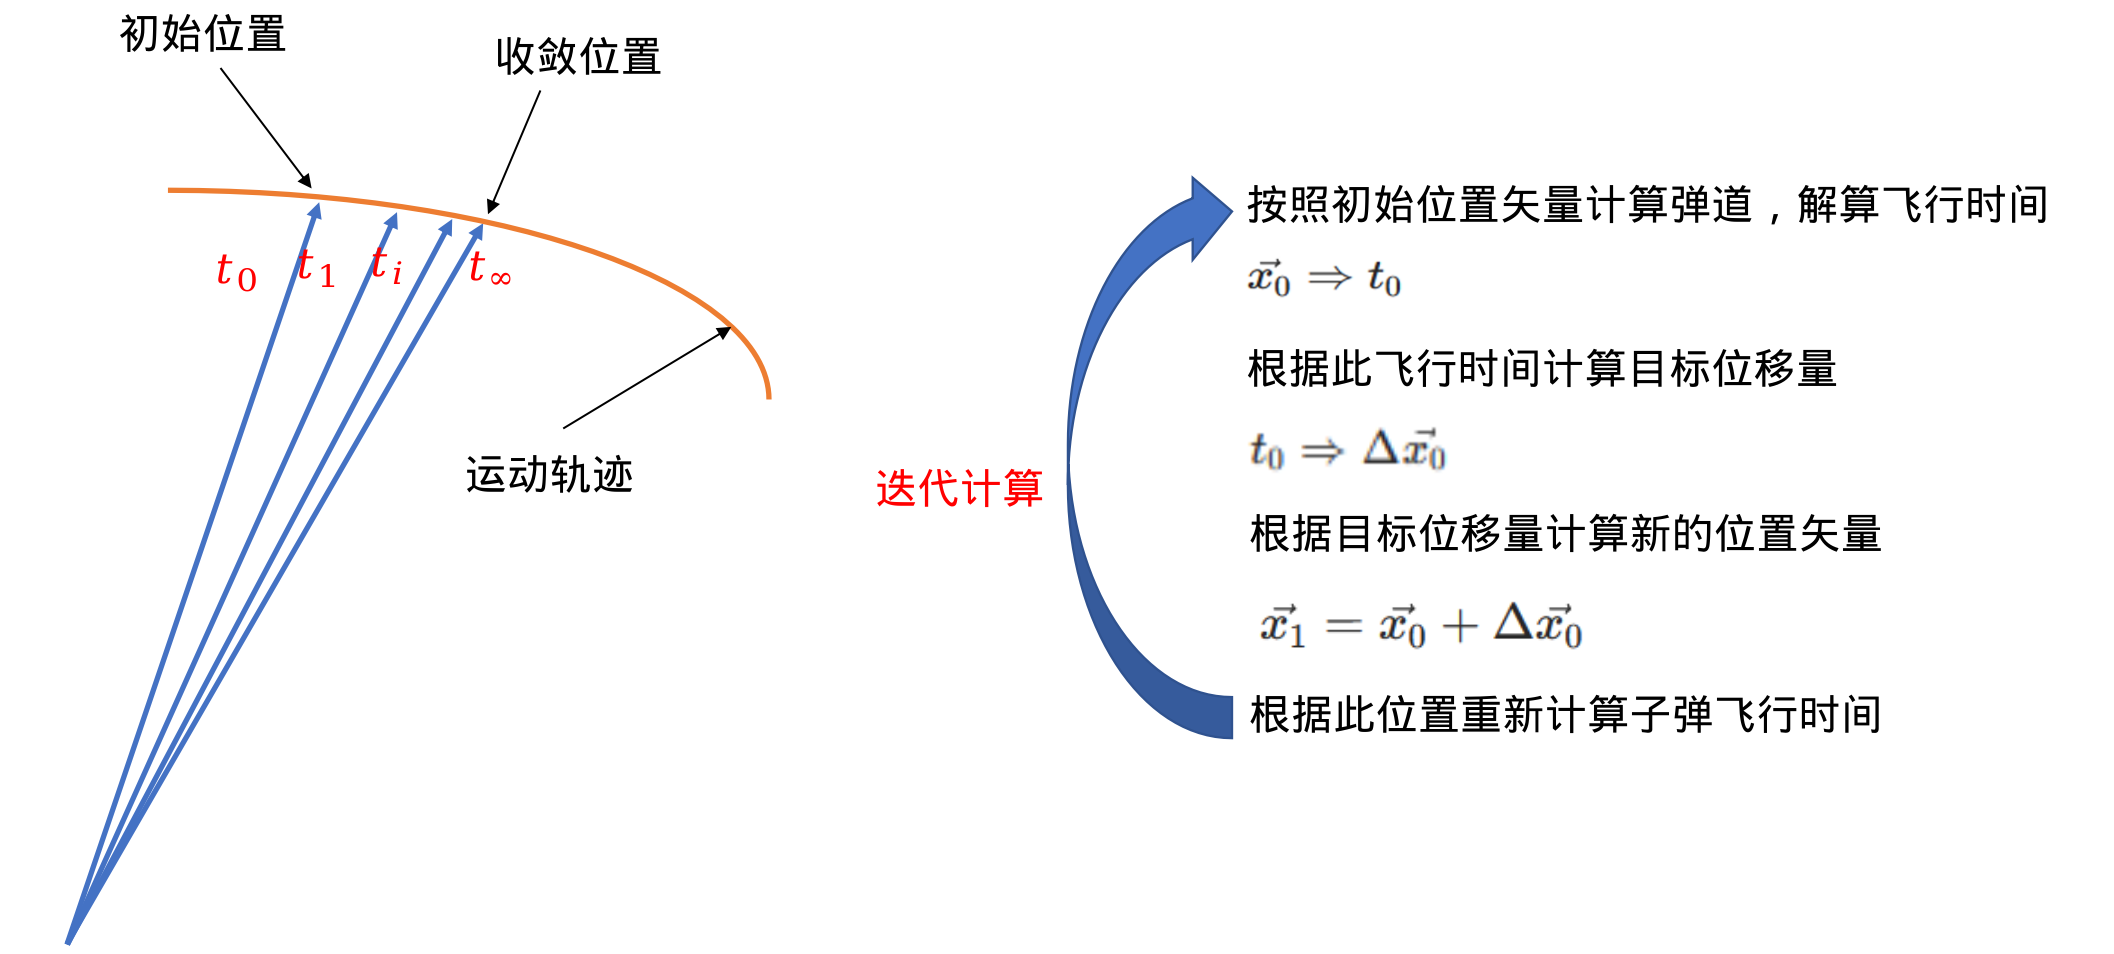
\includegraphics[width=.8\textwidth]{iter.png} 
    \caption{迭代计算过程} 
    \label{迭代计算过程}
\end{figure}

\subsection{弹道轨迹可视化}[Content specification]
使用matplotlib将受空气阻力影响的弹道轨迹和不受空气阻力影响的弹道轨迹可视化。如图\ref{弹道对比}所示,
绿色曲线为不受空气阻力影响的弹道轨迹,红色曲线为受空气阻力影响的弹道轨迹。
\begin{figure}[H]
    \centering
    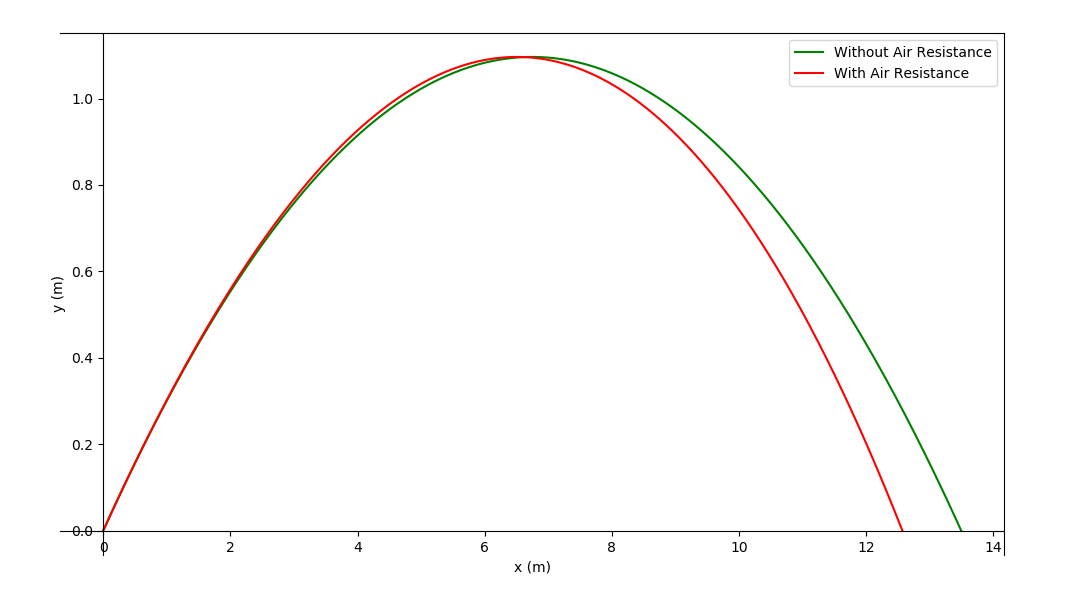
\includegraphics[width=.8\textwidth]{air_resistence_compare.png} 
    \caption{弹道对比图} 
    \label{弹道对比}
\end{figure}






\section{本章小结}[Content specification]
第一小节主要介绍了相机选型、硬件设置和软件设置等方面的知识。
在相机选型方面,需要考虑分辨率、帧率、传感器尺寸和类型、工作温度和防护等级、
以及软件支持等因素。在硬件设置方面,需要注意光圈的设置和成像平面与光心的距离等。
在软件设置方面,需要注意模拟增益的调整和颜色通道增益的选择等。
明确这些方面的知识,可以使相机的使用更加得心应手,也能够为后续的图像处理和算法提供更好的输入数据。
最终选择迈德威视相机,型号为MV-SUA34GC。规格参数在附录2中。

\par
第二小节介绍了如何通过观测固定装甲板惯性下的坐标浮动情况测量通信时延,基于通信实现动态上下位机时间帧对齐,
实现了双机时钟的统一,有利于后续的坐标转换、云台姿态控制等。

\par
第三小节介绍了受空气阻力的弹道迭代计算方法,
包括空气阻力系数的求解和弹丸动力学微分方程的解析解。
针对目标运动情况,提出了数值迭代的解算方法,并给出了迭代计算过程和收敛条件。
最后将受空气阻力与不受空气阻力的弹道轨迹使用matplotlib可视化。
本文提供了一种可行的数值解决方案,对于弹道计算和精确打击目标具有重要意义。
\backmatter
% !Mode:: "TeX:UTF-8" 



\begin{conclusions}

本文介绍了一种基于卡尔曼滤波器的多目标追踪预测算法。
该算法的目的是通过结合高帧率的全局快门相机、基于通信的时间同步协议、
基于传统图像处理算法与深度学习技术结合的目标检测算法、
基于卡尔曼滤波器的运动预测算法
和基于贪心算法的多目标追踪算法等技术手段,实现高效准确的多目标追踪预测任务。

在本文中,我们通过实验验证了该算法的可行性和有效性。实验结果表明,该算法能够在多目标场景下实现高效准确的追踪预测,并且具有较高的实时性和鲁棒性。以下是本文的结论总结:

高帧率的全局快门相机有助于提高多目标追踪预测的准确性。本文采用了高帧率的全局快门相机,
提高了图像的采集频率,从而为目标检测算法提供了更准确的输入。

基于通信的动态时间帧对齐可以保证主从机使用同一时钟源,不仅可以使得识别目标的坐标转换更加准确,
也有利于控制系统在收到滞后控制信息的时候根据时间差补偿,提高了对于动态物体的击打命中率。

基于传统图像处理算法与深度学习技术结合的目标检测算法,
能够高效准确地检测到各种形态的目标。

基于卡尔曼滤波器的运动预测算法可以提高多目标追踪预测的准确性。
本文采用了基于卡尔曼滤波器的运动预测算法,对目标的位置和速度进行预测,从而提高了多目标追踪预测的准确性。

基于贪心算法的多目标追踪算法能够在短时间内得出可接受的解决方案。
本文采用了基于贪心算法的多目标追踪算法,能够在短时间内得出可接受的多目标匹配方案,提高了多目标追踪预测的效率。
综上所述,本文提出的基于卡尔曼滤波器的多目标追踪预测算法,通过结合多种技术手段,实现了高效准确的多
目标追踪预测任务。
该算法具有实现简单、运算速度快、准确度高、鲁棒性强等优点。

然而,该算法仍然存在一些不足之处。
例如,对于极端光照环境、装甲板受遮挡、远距离等情况下,目标检测算法的准确性会受到影响;
对于超机动目标,受限于匀速运动模型的影响,卡尔曼滤波器的预测精度也会受到影响。
因此,未来可以进一步研究如何结合更加先进的目标检测算法
(如端到端直接回归装甲板端点)和更适合机动目标的运动模型(如Singer\cite{2013A}模型),以提高算法的鲁棒性和精度。



\end{conclusions}
   % 结论
\bibliographystyle{gbt7714-numerical}
%%%%%%%%%%%%%%%%%%%%%%%%%%%%%%%%%%%%%%%%%%%%%%%%%%%%%%%%%%%%%%%%%%%%%%%%%%%%%%%%
%-- 注意:以下本硕博、博后书序不一致 --%
%%%%%%%%%%%%%%%%%%%%%%%%%%%%%%%%%%%%%%%%%%%%%%%%%%%%%%%%%%%%%%%%%%%%%%%%%%%%%%%%
% 本科书序(哈尔滨、深圳校区)
%%%%%%%%%%%%%%%%%%%%%%%%%%%%%%%%%%%%%%%%%%%%%%%%%%%%%%%%%%%%%%%%%%%%%%%%%%%%%%%%
% \bibliography{reference} % 参考文献
% \authorization %授权
% % \authorization[scan.pdf] %添加扫描页的命令,与上互斥
% % !Mode:: "TeX:UTF-8"
\begin{acknowledgements}
衷心感谢导师赵明航教授对本人的精心指导。他的言传身教将使我终生受益。
感谢HERO竞技机器人队,我不仅学到了理论,锻炼了工程能力,还认识到了一群非常纯粹、追求极致技术的人。做
有实践精神的梦想家!

感谢哈工大\LaTeX\ 论文模板\hithesis\ !

\end{acknowledgements}
 %致谢
% \begin{appendix}%附录
% \chapter{外文资料原文}
\label{cha:engorg}

\title{The title of the English paper}

\textbf{Abstract:} As one of the most widely used techniques in operations
research, \emph{ mathematical programming} is defined as a means of maximizing a
quantity known as \emph{bjective function}, subject to a set of constraints
represented by equations and inequalities. Some known subtopics of mathematical
programming are linear programming, nonlinear programming, multiobjective
programming, goal programming, dynamic programming, and multilevel
programming$^{[1]}$.

It is impossible to cover in a single chapter every concept of mathematical
programming. This chapter introduces only the basic concepts and techniques of
mathematical programming such that readers gain an understanding of them
throughout the book$^{[2,3]}$.


\section{Single-Objective Programming}
The general form of single-objective programming (SOP) is written
as follows,
\begin{equation}\tag*{(123)} % 如果附录中的公式不想让它出现在公式索引中,那就请
                             % 用 \tag*{xxxx}
\left\{\begin{array}{l}
\max \,\,f(x)\\[0.1 cm]
\mbox{subject to:} \\ [0.1 cm]
\qquad g_j(x)\le 0,\quad j=1,2,\cdots,p
\end{array}\right.
\end{equation}
which maximizes a real-valued function $f$ of
$x=(x_1,x_2,\cdots,x_n)$ subject to a set of constraints.

\newtheorem{mpdef}{Definition}[chapter]
\begin{mpdef}
In SOP, we call $x$ a decision vector, and
$x_1,x_2,\cdots,x_n$ decision variables. The function
$f$ is called the objective function. The set
\begin{equation}\tag*{(456)} % 这里同理,其它不再一一指定。
S=\left\{x\in\Re^n\bigm|g_j(x)\le 0,\,j=1,2,\cdots,p\right\}
\end{equation}
is called the feasible set. An element $x$ in $S$ is called a
feasible solution.
\end{mpdef}

\newtheorem{mpdefop}[mpdef]{Definition}
\begin{mpdefop}
A feasible solution $x^*$ is called the optimal
solution of SOP if and only if
\begin{equation}
f(x^*)\ge f(x)
\end{equation}
for any feasible solution $x$.
\end{mpdefop}

One of the outstanding contributions to mathematical programming was known as
the Kuhn-Tucker conditions\ref{eq:ktc}. In order to introduce them, let us give
some definitions. An inequality constraint $g_j(x)\le 0$ is said to be active at
a point $x^*$ if $g_j(x^*)=0$. A point $x^*$ satisfying $g_j(x^*)\le 0$ is said
to be regular if the gradient vectors $\nabla g_j(x)$ of all active constraints
are linearly independent.

Let $x^*$ be a regular point of the constraints of SOP and assume that all the
functions $f(x)$ and $g_j(x),j=1,2,\cdots,p$ are differentiable. If $x^*$ is a
local optimal solution, then there exist Lagrange multipliers
$\lambda_j,j=1,2,\cdots,p$ such that the following Kuhn-Tucker conditions hold,
\begin{equation}
\label{eq:ktc}
\left\{\begin{array}{l}
    \nabla f(x^*)-\sum\limits_{j=1}^p\lambda_j\nabla g_j(x^*)=0\\[0.3cm]
    \lambda_jg_j(x^*)=0,\quad j=1,2,\cdots,p\\[0.2cm]
    \lambda_j\ge 0,\quad j=1,2,\cdots,p.
\end{array}\right.
\end{equation}
If all the functions $f(x)$ and $g_j(x),j=1,2,\cdots,p$ are convex and
differentiable, and the point $x^*$ satisfies the Kuhn-Tucker conditions
(\ref{eq:ktc}), then it has been proved that the point $x^*$ is a global optimal
solution of SOP.

\subsection{Linear Programming}
\label{sec:lp}

If the functions $f(x),g_j(x),j=1,2,\cdots,p$ are all linear, then SOP is called
a {\em linear programming}.

The feasible set of linear is always convex. A point $x$ is called an extreme
point of convex set $S$ if $x\in S$ and $x$ cannot be expressed as a convex
combination of two points in $S$. It has been shown that the optimal solution to
linear programming corresponds to an extreme point of its feasible set provided
that the feasible set $S$ is bounded. This fact is the basis of the {\em simplex
  algorithm} which was developed by Dantzig as a very efficient method for
solving linear programming.
\begin{table}[ht]
\centering
  \centering
  \caption*{Table~1\hskip1em This is an example for manually numbered table, which
    would not appear in the list of tables}
  \label{tab:badtabular2}
  \begin{tabular}[c]{|m{1.5cm}|c|c|c|c|c|c|}\hline
    \multicolumn{2}{|c|}{Network Topology} & \# of nodes &
    \multicolumn{3}{c|}{\# of clients} & Server \\\hline
    GT-ITM & Waxman Transit-Stub & 600 &
    \multirow{2}{2em}{2\%}&
    \multirow{2}{2em}{10\%}&
    \multirow{2}{2em}{50\%}&
    \multirow{2}{1.2in}{Max. Connectivity}\\\cline{1-3}
    \multicolumn{2}{|c|}{Inet-2.1} & 6000 & & & &\\\hline
    & \multicolumn{2}{c|}{ABCDEF} &\multicolumn{4}{c|}{} \\\hline
\end{tabular}
\end{table}

Roughly speaking, the simplex algorithm examines only the extreme points of the
feasible set, rather than all feasible points. At first, the simplex algorithm
selects an extreme point as the initial point. The successive extreme point is
selected so as to improve the objective function value. The procedure is
repeated until no improvement in objective function value can be made. The last
extreme point is the optimal solution.

\subsection{Nonlinear Programming}

If at least one of the functions $f(x),g_j(x),j=1,2,\cdots,p$ is nonlinear, then
SOP is called a {\em nonlinear programming}.

A large number of classical optimization methods have been developed to treat
special-structural nonlinear programming based on the mathematical theory
concerned with analyzing the structure of problems.

Now we consider a nonlinear programming which is confronted solely with
maximizing a real-valued function with domain $\Re^n$.  Whether derivatives are
available or not, the usual strategy is first to select a point in $\Re^n$ which
is thought to be the most likely place where the maximum exists. If there is no
information available on which to base such a selection, a point is chosen at
random. From this first point an attempt is made to construct a sequence of
points, each of which yields an improved objective function value over its
predecessor. The next point to be added to the sequence is chosen by analyzing
the behavior of the function at the previous points. This construction continues
until some termination criterion is met. Methods based upon this strategy are
called {\em ascent methods}, which can be classified as {\em direct methods},
{\em gradient methods}, and {\em Hessian methods} according to the information
about the behavior of objective function $f$. Direct methods require only that
the function can be evaluated at each point. Gradient methods require the
evaluation of first derivatives of $f$. Hessian methods require the evaluation
of second derivatives. In fact, there is no superior method for all
problems. The efficiency of a method is very much dependent upon the objective
function.

\subsection{Integer Programming}

{\em Integer programming} is a special mathematical programming in which all of
the variables are assumed to be only integer values. When there are not only
integer variables but also conventional continuous variables, we call it {\em
  mixed integer programming}. If all the variables are assumed either 0 or 1,
then the problem is termed a {\em zero-one programming}. Although integer
programming can be solved by an {\em exhaustive enumeration} theoretically, it
is impractical to solve realistically sized integer programming problems. The
most successful algorithm so far found to solve integer programming is called
the {\em branch-and-bound enumeration} developed by Balas (1965) and Dakin
(1965). The other technique to integer programming is the {\em cutting plane
  method} developed by Gomory (1959).

\hfill\textit{Uncertain Programming\/}\quad(\textsl{BaoDing Liu, 2006.2})

\section*{References}
\noindent{\itshape NOTE: These references are only for demonstration. They are
  not real citations in the original text.}

\begin{translationbib}
\item Donald E. Knuth. The \TeX book. Addison-Wesley, 1984. ISBN: 0-201-13448-9
\item Paul W. Abrahams, Karl Berry and Kathryn A. Hargreaves. \TeX\ for the
  Impatient. Addison-Wesley, 1990. ISBN: 0-201-51375-7
\item David Salomon. The advanced \TeX book.  New York : Springer, 1995. ISBN:0-387-94556-3
\end{translationbib}

\chapter{外文资料的调研阅读报告或书面翻译}

\title{英文资料的中文标题}

{\heiti 摘要:} 本章为外文资料翻译内容。如果有摘要可以直接写上来,这部分好像没有
明确的规定。

\section{单目标规划}
北冥有鱼,其名为鲲。鲲之大,不知其几千里也。化而为鸟,其名为鹏。鹏之背,不知其几
千里也。怒而飞,其翼若垂天之云。是鸟也,海运则将徙于南冥。南冥者,天池也。
\begin{equation}\tag*{(123)}
 p(y|\mathbf{x}) = \frac{p(\mathbf{x},y)}{p(\mathbf{x})}=
\frac{p(\mathbf{x}|y)p(y)}{p(\mathbf{x})}
\end{equation}

吾生也有涯,而知也无涯。以有涯随无涯,殆已!已而为知者,殆而已矣!为善无近名,为
恶无近刑,缘督以为经,可以保身,可以全生,可以养亲,可以尽年。

\subsection{线性规划}
庖丁为文惠君解牛,手之所触,肩之所倚,足之所履,膝之所倚,砉然响然,奏刀騞然,莫
不中音,合于桑林之舞,乃中经首之会。
\begin{table}[ht]
\centering
  \centering
  \caption*{表~1\hskip1em 这是手动编号但不出现在索引中的一个表格例子}
  \label{tab:badtabular3}
  \begin{tabular}[c]{|m{1.5cm}|c|c|c|c|c|c|}\hline
    \multicolumn{2}{|c|}{Network Topology} & \# of nodes &
    \multicolumn{3}{c|}{\# of clients} & Server \\\hline
    GT-ITM & Waxman Transit-Stub & 600 &
    \multirow{2}{2em}{2\%}&
    \multirow{2}{2em}{10\%}&
    \multirow{2}{2em}{50\%}&
    \multirow{2}{1.2in}{Max. Connectivity}\\\cline{1-3}
    \multicolumn{2}{|c|}{Inet-2.1} & 6000 & & & &\\\hline
    & \multicolumn{2}{c|}{ABCDEF} &\multicolumn{4}{c|}{} \\\hline
\end{tabular}
\end{table}

文惠君曰:“嘻,善哉!技盖至此乎?”庖丁释刀对曰:“臣之所好者道也,进乎技矣。始臣之
解牛之时,所见无非全牛者;三年之后,未尝见全牛也;方今之时,臣以神遇而不以目视,
官知止而神欲行。依乎天理,批大郤,导大窾,因其固然。技经肯綮之未尝,而况大坬乎!
良庖岁更刀,割也;族庖月更刀,折也;今臣之刀十九年矣,所解数千牛矣,而刀刃若新发
于硎。彼节者有间而刀刃者无厚,以无厚入有间,恢恢乎其于游刃必有余地矣。是以十九年
而刀刃若新发于硎。虽然,每至于族,吾见其难为,怵然为戒,视为止,行为迟,动刀甚微,
謋然已解,如土委地。提刀而立,为之而四顾,为之踌躇满志,善刀而藏之。”

文惠君曰:“善哉!吾闻庖丁之言,得养生焉。”


\subsection{非线性规划}
孔子与柳下季为友,柳下季之弟名曰盗跖。盗跖从卒九千人,横行天下,侵暴诸侯。穴室枢
户,驱人牛马,取人妇女。贪得忘亲,不顾父母兄弟,不祭先祖。所过之邑,大国守城,小
国入保,万民苦之。孔子谓柳下季曰:“夫为人父者,必能诏其子;为人兄者,必能教其弟。
若父不能诏其子,兄不能教其弟,则无贵父子兄弟之亲矣。今先生,世之才士也,弟为盗
跖,为天下害,而弗能教也,丘窃为先生羞之。丘请为先生往说之。”

柳下季曰:“先生言为人父者必能诏其子,为人兄者必能教其弟,若子不听父之诏,弟不受
兄之教,虽今先生之辩,将奈之何哉?且跖之为人也,心如涌泉,意如飘风,强足以距敌,
辩足以饰非。顺其心则喜,逆其心则怒,易辱人以言。先生必无往。”

孔子不听,颜回为驭,子贡为右,往见盗跖。

\subsection{整数规划}
盗跖乃方休卒徒大山之阳,脍人肝而餔之。孔子下车而前,见谒者曰:“鲁人孔丘,闻将军
高义,敬再拜谒者。”谒者入通。盗跖闻之大怒,目如明星,发上指冠,曰:“此夫鲁国之
巧伪人孔丘非邪?为我告之:尔作言造语,妄称文、武,冠枝木之冠,带死牛之胁,多辞缪
说,不耕而食,不织而衣,摇唇鼓舌,擅生是非,以迷天下之主,使天下学士不反其本,妄
作孝弟,而侥幸于封侯富贵者也。子之罪大极重,疾走归!不然,我将以子肝益昼餔之膳。”


\chapter{其它附录}
前面两个附录主要是给本科生做例子。其它附录的内容可以放到这里,当然如果你愿意,可
以把这部分也放到独立的文件中,然后将其到主文件中。
%本科生翻译论文
% \end{appendix}
%%%%%%%%%%%%%%%%%%%%%%%%%%%%%%%%%%%%%%%%%%%%%%%%%%%%%%%%%%%%%%%%%%%%%%%%%%%%%%%%
% 本科书序(威海校区)
%%%%%%%%%%%%%%%%%%%%%%%%%%%%%%%%%%%%%%%%%%%%%%%%%%%%%%%%%%%%%%%%%%%%%%%%%%%%%%%%
\bibliography{reference} % 参考文献
\authorization %授权 
% \authorization[scan.pdf] %添加扫描页的命令,与上互斥
% !Mode:: "TeX:UTF-8"
\begin{acknowledgements}
衷心感谢导师赵明航教授对本人的精心指导。他的言传身教将使我终生受益。
感谢HERO竞技机器人队,我不仅学到了理论,锻炼了工程能力,还认识到了一群非常纯粹、追求极致技术的人。做
有实践精神的梦想家!

感谢哈工大\LaTeX\ 论文模板\hithesis\ !

\end{acknowledgements}
 %致谢
\begin{appendix}%附录


\chapter[程序开发使用工具]{程序开发所使用工具}[Harbin Institute of Technology Postgraduate Dissertation Writing Specifications]

\section{代码智能提示工具}[Content specification]
clangd是一个基于Clang的C++语言服务器,它提供了丰富的C++代码补全、跳转、重构、文档查询等功能,
是现代化C++开发环境的重要组成部分。它使用了LLVM和Clang提供的强大的代码分析功能,
并通过LSP(Language Server Protocol)与各种编辑器集成,包括VSCode、Sublime、Emacs等。

clangd的主要功能包括:

\begin{itemize}[itemindent=2em]
\item 代码补全:clangd可以为用户提供即时的代码补全功能,包括类、函数、变量等。它可以根据上下文,自动推断用户的意图,并提供最合适的代码补全建议。

\item 跳转:clangd可以让用户快速跳转到类、函数、变量的定义处,方便用户查看源代码。

\item 重构:clangd可以帮助用户进行一些重构操作,比如修改函数签名、移动函数等。

\item 文档查询:clangd可以帮助用户查看代码文档,包括函数说明、参数说明、返回值说明等。

\item 错误提示:clangd可以帮助用户发现代码错误,并给出相应的提示,方便用户快速定位和修复代码问题。
\end{itemize}


\section{静态代码分析工具}[Content specification]
clang-tidy是一个基于Clang的静态代码分析工具,可以自动检查代码中的一些潜在问题,
并给出相应的建议和修复方案。它使用了LLVM和Clang提供的强大的代码分析功能,
并提供了一系列的检查器,用于检测常见的代码问题,比如空指针访问、未初始化变量使用、内存泄露等。

clang-tidy的主要功能包括:
\begin{itemize}[itemindent=2em]

\item 自动检测:clang-tidy可以自动检测代码中的一些潜在问题,并给出相应的建议和修复方案。

\item 多种检查器:clang-tidy提供了多种检查器,可以检测常见的代码问题,比如空指针访问、未初始化变量使用、内存泄露等。

\item 自定义检查:clang-tidy还支持自定义检查器,用户可以根据自己的需求编写自己的检查器。

\item IDE集成:clang-tidy可以与多种IDE(Integrated Development Environment,集成开发环境)集成,比如VSCode、Clion等。

\item 自动修复:clang-tidy还支持自动修复代码中的一些问题,减少开发者手动修改代码的工作量。
\end{itemize}


\section{程序性能分析工具}[Content specification]
使用gperftools分析程序寻找速度瓶颈,实现针对性优化。
gperftools是一个Google开发的性能优化工具集,用于帮助开发者优化应用程序的内存和CPU使用效率。
它包含了多个工具,如CPU Profiler、Heap Profiler、Profiler GUI等,
这些工具可以帮助开发者在运行时识别和解决应用程序中的性能问题。

CPU Profiler是gperftools工具集中的一个工具,它的原理是通过采样技术来识别和分析应用程序中的CPU使用情况。具体来说,CPU Profiler会在应用程序运行时以固定的时间间隔对CPU进行采样,记录下此时CPU所在的程序计数器值(PC值)和调用栈信息。

PC值是指CPU当前所执行的指令的内存地址,通过记录PC值可以知道程序正在执行哪个函数。而调用栈则是指当前函数的调用关系,包括该函数的调用者、被调用者等信息。通过采样得到的PC值和调用栈信息,CPU Profiler可以计算出每个函数的CPU使用时间和调用次数,从而得出应用程序中每个函数的CPU使用情况。

在分析采样数据时,CPU Profiler会使用一些统计技术,如调用图、热点函数列表等,来帮助开发者快速定位和分析CPU密集型的函数,并进行优化。此外,CPU Profiler还可以生成调用图和火焰图等可视化工具,方便开发者更直观地查看和分析采样数据。
\section{内存泄露分析工具}[Content specification]
% 使用Valgrind检测程序在运行中可能出现的内存泄露情况。
Valgrind是一个用于检测程序内存管理问题的开源工具集,支持C/C++等多种编程语言。
它可以帮助开发者检测程序的内存泄漏、
使用未初始化的变量、访问越界、使用已释放的内存等问题。
Valgrind通过模拟运行程序,捕捉所有的内存操作,并且能够检测到许多难以发现的内存问题。

Valgrind包括多个工具,其中最常用的是Memcheck。
Memcheck可以检测程序中的内存泄漏、读写越界、使用未初始化的变量等问题,
它可以在不修改程序源代码的情况下运行程序并捕捉这些问题。
当Memcheck检测到问题时,它会输出详细的错误信息,包括错误发生的位置和类型。
除了Memcheck之外,Valgrind还包括其他的工具,
如Cachegrind、Helgrind等,可以用于检测程序的性能和线程安全性问题。


\chapter[MV-SUA34GC相机参数]{MV-SUA34GC相机参数}[Harbin Institute of Technology Postgraduate Dissertation Writing Specifications]
\begin{figure}[htbp]
    \centering
    \includegraphics[page=2, scale=0.6]{back/camera.pdf}
\end{figure}

\end{appendix}
%%%%%%%%%%%%%%%%%%%%%%%%%%%%%%%%%%%%%%%%%%%%%%%%%%%%%%%%%%%%%%%%%%%%%%%%%%%%%%%%
% 硕博书序
%%%%%%%%%%%%%%%%%%%%%%%%%%%%%%%%%%%%%%%%%%%%%%%%%%%%%%%%%%%%%%%%%%%%%%%%%%%%%%%%
% \bibliography{reference} % 参考文献
% \begin{appendix}%附录
% % -*-coding: utf-8 -*-
%%%%%%%%%%%%%%%%%%%%%%%%%%%%%%%%%%%%%%%%%%%%%%%%%%%%%%%%%
\chapter{带章节的附录}[Full Appendix]%
完整的附录内容,包含章节,公式,图表等

%%%%%%%%%%%%%%%%%%%%%%%%%%%%%%%%%%%%%%%%%%%%%%%%%%%%%%%%%
\section{附录节的内容}[Section in Appendix]
这是附录的节的内容

附录中图的示例:
\begin{figure}[htbp]
\centering
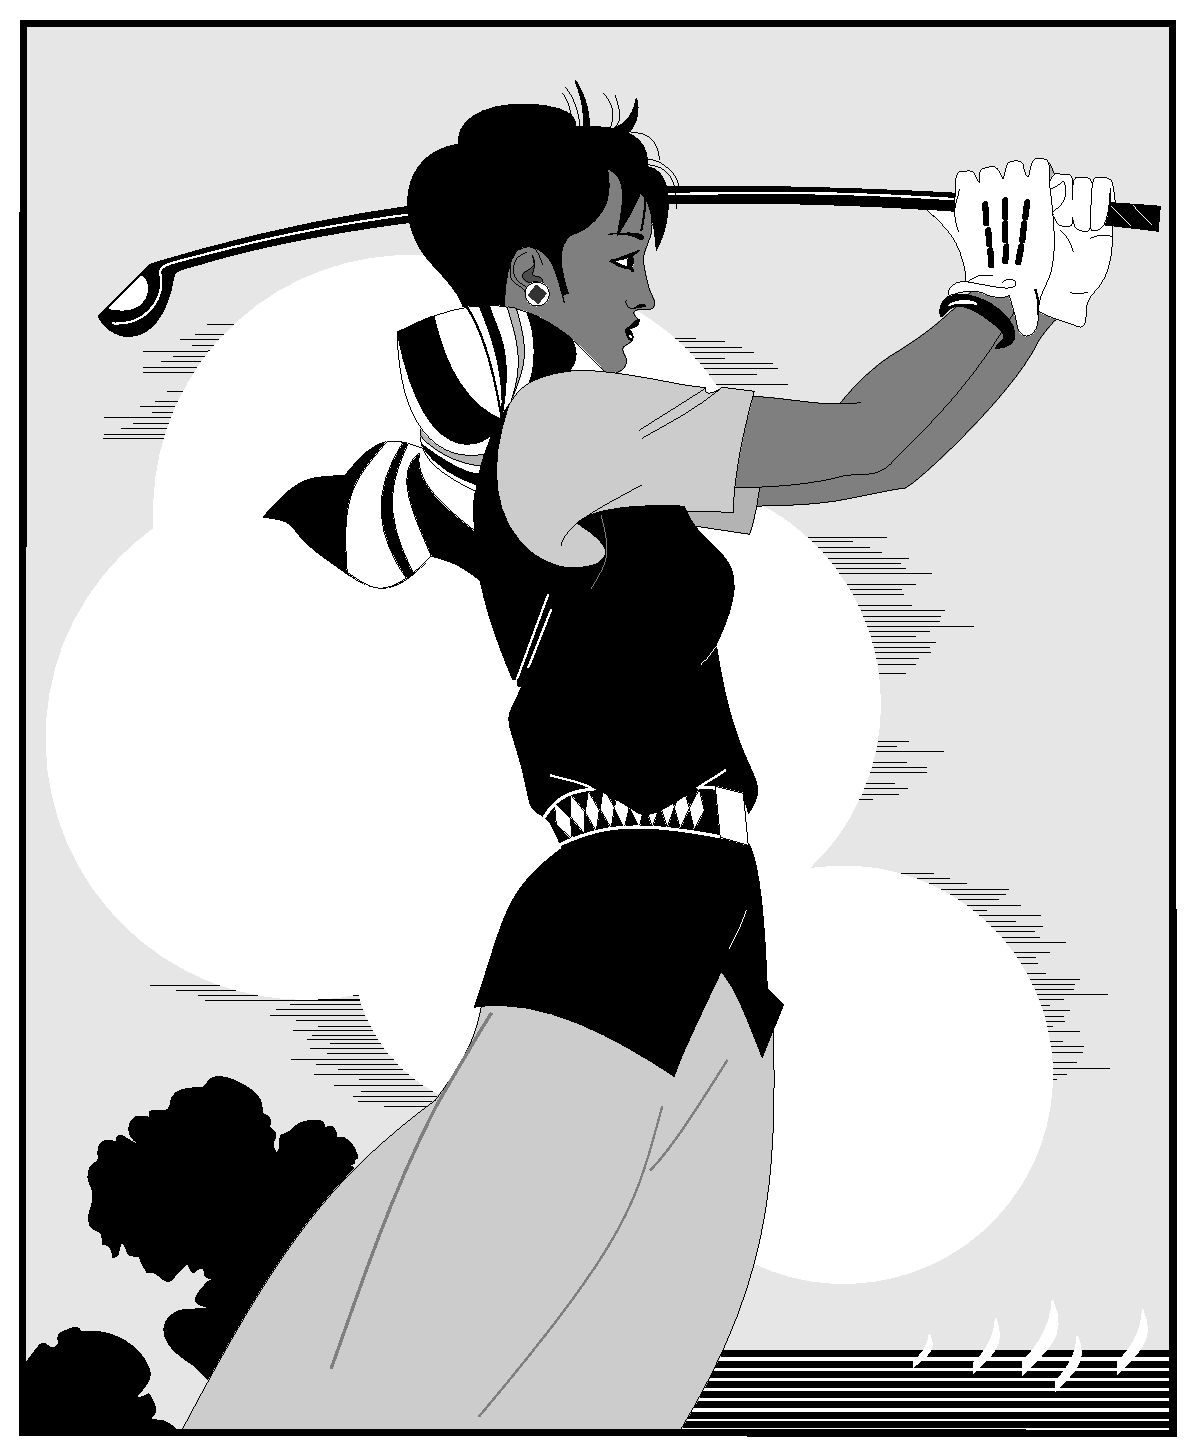
\includegraphics[width = 0.4\textwidth]{golfer}
%\bicaption[golfer5]{}{\xiaosi[0]打高尔夫球的人}{Fig.$\!$}{The person playing golf}\vspace{-1em}
\caption{\xiaosi[0]打高尔夫球的人}
\end{figure}

附录中公式的示例:
\begin{align}
a & = b \times c \\
E & = m c^2
\label{eq}
\end{align}

\chapter{这个星球上最好的免费Linux软件列表}[List of the Best Linux Software in our Planet]
\section{系统}

\href{http://fvwm.org/}{FVWM 自从上世纪诞生以来,此星球最强大的窗口管理器。}
推荐基于FVWM的桌面设计hifvwm:\href{https://github.com/dustincys/hifvwm}{https://github.com/dustincys/hifvwm}。

\subsection{hifvwm的优点}

\begin{enumerate}
	\item 即使打开上百个窗口也不会“蒙圈”。计算机性能越来越强大,窗口任务的管理必须要升级到打怪兽级别。
	\item 自动同步Bing搜索主页的壁纸。每次电脑开机,午夜零点自动更新,用户
		也可以手动更新,从此审美再也不疲劳。
	\item 切换窗口自动聚焦到最上面的窗口。使用键盘快捷键切换窗口时候,减少
		操作过程,自动聚焦到目标窗口。这一特性是虚拟窗口必须的人性化设
		计。
	\item 类似window右下角的功能的最小化窗口来显示桌面的功能此处类似
		win7/win10,实现在一个桌面之内操作多个任务。
	\item 任务栏结合标题栏。采用任务栏和标题栏结合,节省空间。
	\item 同类窗口切换。可以在同类窗口之内类似alt-tab的方式切换。
	\item ……
\end{enumerate}

\section{其他}

\href{https://github.com/goldendict/goldendict}{goldendict 星球最强大的桌面字典。}

\href{https://github.com/yarrick/iodine}{iodine,“HIT-WLAN + 锐捷”时代的福音。}

\href{http://www.aircrack-ng.org/}{aircrack,Wifi“安全性评估”工具。}

\href{https://www.ledger-cli.org/}{ledger,前“金融区块链”时代最好的复式记账系统。}

\href{https://orgmode.org/}{orgmode,最强大的笔记系统,从来没有之一。}

\href{https://www.jianguoyun.com/}{坚果云,国内一款支持WebDav的云盘系统,国内真正的云盘没有之一。}

\href{http://www.mutt.org/}{mutt, ``All mail clients suck. This one just sucks less.''}

\section{vim}
实现中英文每一句一行,以及实现每一句折叠断行的简单正则式,tex源码更加乖乖。
\begin{lstlisting}
vnoremap <leader>fae J:s/[.!?]\zs\s\+/\="\r".matchstr(getline('.'), '^\s*')/g<CR>
vnoremap <leader>fac J:s/[。!?]/\=submatch(0)."\n".matchstr(getline('.'), '^\s*')/g<CR>
vnoremap <leader>fle :!fmt -80 -s<CR>
\end{lstlisting}

% \end{appendix}
% % !Mode:: "TeX:UTF-8" 
\begin{publication}
\noindent\textbf{发表的相关论文}
\begin{publist}
\item	XXX,XXX. Static Oxidation Model of Al-Mg/C Dissipation Thermal Protection Materials[J]. Rare Metal Materials and Engineering, 2010, 39(Suppl. 1): 520-524.(SCI~收录,IDS号为~669JS,IF=0.16)
\item XXX,XXX. 精密超声振动切削单晶铜的计算机仿真研究[J]. 系统仿真学报,2007,19(4):738-741,753.(EI~收录号:20071310514841)
\item XXX,XXX. 局部多孔质气体静压轴向轴承静态特性的数值求解[J]. 摩擦学学报,2007(1):68-72.(EI~收录号:20071510544816)
\item XXX,XXX. 硬脆光学晶体材料超精密切削理论研究综述[J]. 机械工程学报,2003,39(8):15-22.(EI~收录号:2004088028875)
\item XXX,XXX. 基于遗传算法的超精密切削加工表面粗糙度预测模型的参数辨识以及切削参数优化[J]. 机械工程学报,2005,41(11):158-162.(EI~收录号:2006039650087)
\item XXX,XXX. Discrete Sliding Mode Cintrok with Fuzzy Adaptive Reaching Law on 6-PEES Parallel Robot[C]. Intelligent System Design and Applications, Jinan, 2006: 649-652.(EI~收录号:20073210746529)
\end{publist}

\noindent\textbf{(二)申请及已获得的专利(无专利时此项不必列出)}
\begin{publist}
\item XXX,XXX. 一种温热外敷药制备方案:中国,88105607.3[P]. 1989-07-26.
\end{publist}

\noindent\textbf{(三)参与的科研项目及获奖情况}
\begin{publist}
\item	XXX,XXX. XX~气体静压轴承技术研究, XX~省自然科学基金项目.课题编号:XXXX.
\item XXX,XXX. XX~静载下预应力混凝土房屋结构设计统一理论. 黑江省科学技术二等奖, 2007.
\end{publist}
%\vfill
%\hangafter=1\hangindent=2em\noindent
%\setlength{\parindent}{2em}
\end{publication}
    % 所发文章
% \begin{ceindex}
  %如果想要手动加索引,注释掉以下这一样,用wordlist环境
\printsubindex*
\end{ceindex}
    % 索引, 根据自己的情况添加或者不添加,选择自动添加或者手工添加。
% \authorization %授权
% %\authorization[scan.pdf] %添加扫描页的命令,与上互斥
% % !Mode:: "TeX:UTF-8"
\begin{acknowledgements}
衷心感谢导师赵明航教授对本人的精心指导。他的言传身教将使我终生受益。
感谢HERO竞技机器人队,我不仅学到了理论,锻炼了工程能力,还认识到了一群非常纯粹、追求极致技术的人。做
有实践精神的梦想家!

感谢哈工大\LaTeX\ 论文模板\hithesis\ !

\end{acknowledgements}
 %致谢
% % !Mode:: "TeX:UTF-8" 

\begin{resume}
XXXX~年~XX~月~XX~日出生于~XXXX。

XXXX~年~XX~月考入~XX~大学~XX~院(系)XX~专业,XXXX~年~XX~月本科毕业并获得~XX~学学士学位。

XXXX~年~XX~月------XXXX~年~XX~月在~XX~大学~XX~院(系)XX~学科学习并获得~XX~学硕士学位。

XXXX~年~XX~月------XXXX~年~XX~月在~XX~大学~XX~院(系)XX~学科学习并获得~XX~学博士学位。

获奖情况:如获三好学生、优秀团干部、X~奖学金等(不含科研学术获奖)。

工作经历:

\textbf{( 除全日制硕士生以外,其余学生均应增列此项。个人简历一般应包含教育经历和工作经历。)}
\end{resume}
          % 博士学位论文有个人简介
%%%%%%%%%%%%%%%%%%%%%%%%%%%%%%%%%%%%%%%%%%%%%%%%%%%%%%%%%%%%%%%%%%%%%%%%%%%%%%%%
% 博后书序
%%%%%%%%%%%%%%%%%%%%%%%%%%%%%%%%%%%%%%%%%%%%%%%%%%%%%%%%%%%%%%%%%%%%%%%%%%%%%%%%
% \bibliography{reference} % 参考文献
% % !Mode:: "TeX:UTF-8"
\begin{acknowledgements}
衷心感谢导师赵明航教授对本人的精心指导。他的言传身教将使我终生受益。
感谢HERO竞技机器人队,我不仅学到了理论,锻炼了工程能力,还认识到了一群非常纯粹、追求极致技术的人。做
有实践精神的梦想家!

感谢哈工大\LaTeX\ 论文模板\hithesis\ !

\end{acknowledgements}
 %致谢
% % !Mode:: "TeX:UTF-8" 

\begin{doctorpublication}
\noindent\textbf{(一)发表的学术论文}
\begin{publist}
\item	XXX,XXX. Static Oxidation Model of Al-Mg/C Dissipation Thermal Protection Materials[J]. Rare Metal Materials and Engineering, 2010, 39(Suppl. 1): 520-524.(SCI~收录,IDS号为~669JS,IF=0.16)
\item XXX,XXX. 精密超声振动切削单晶铜的计算机仿真研究[J]. 系统仿真学报,2007,19(4):738-741,753.(EI~收录号:20071310514841)
\item XXX,XXX. 局部多孔质气体静压轴向轴承静态特性的数值求解[J]. 摩擦学学报,2007(1):68-72.(EI~收录号:20071510544816)
\item XXX,XXX. 硬脆光学晶体材料超精密切削理论研究综述[J]. 机械工程学报,2003,39(8):15-22.(EI~收录号:2004088028875)
\item XXX,XXX. 基于遗传算法的超精密切削加工表面粗糙度预测模型的参数辨识以及切削参数优化[J]. 机械工程学报,2005,41(11):158-162.(EI~收录号:2006039650087)
\item XXX,XXX. Discrete Sliding Mode Cintrok with Fuzzy Adaptive Reaching Law on 6-PEES Parallel Robot[C]. Intelligent System Design and Applications, Jinan, 2006: 649-652.(EI~收录号:20073210746529)
\end{publist}

\noindent\textbf{(二)申请及已获得的专利(无专利时此项不必列出)}
\begin{publist}
\item XXX,XXX. 一种温热外敷药制备方案:中国,88105607.3[P]. 1989-07-26.
\end{publist}

\noindent\textbf{(三)参与的科研项目及获奖情况}
\begin{publist}
\item	XXX,XXX. XX~气体静压轴承技术研究, XX~省自然科学基金项目.课题编号:XXXX.
\item XXX,XXX. XX~静载下预应力混凝土房屋结构设计统一理论. 黑江省科学技术二等奖, 2007.
\end{publist}
%\vfill
%\hangafter=1\hangindent=2em\noindent
%\setlength{\parindent}{2em}
\end{doctorpublication}
    % 所发文章
% % !Mode:: "TeX:UTF-8" 
\begin{publication}
\noindent\textbf{发表的相关论文}
\begin{publist}
\item	XXX,XXX. Static Oxidation Model of Al-Mg/C Dissipation Thermal Protection Materials[J]. Rare Metal Materials and Engineering, 2010, 39(Suppl. 1): 520-524.(SCI~收录,IDS号为~669JS,IF=0.16)
\item XXX,XXX. 精密超声振动切削单晶铜的计算机仿真研究[J]. 系统仿真学报,2007,19(4):738-741,753.(EI~收录号:20071310514841)
\item XXX,XXX. 局部多孔质气体静压轴向轴承静态特性的数值求解[J]. 摩擦学学报,2007(1):68-72.(EI~收录号:20071510544816)
\item XXX,XXX. 硬脆光学晶体材料超精密切削理论研究综述[J]. 机械工程学报,2003,39(8):15-22.(EI~收录号:2004088028875)
\item XXX,XXX. 基于遗传算法的超精密切削加工表面粗糙度预测模型的参数辨识以及切削参数优化[J]. 机械工程学报,2005,41(11):158-162.(EI~收录号:2006039650087)
\item XXX,XXX. Discrete Sliding Mode Cintrok with Fuzzy Adaptive Reaching Law on 6-PEES Parallel Robot[C]. Intelligent System Design and Applications, Jinan, 2006: 649-652.(EI~收录号:20073210746529)
\end{publist}

\noindent\textbf{(二)申请及已获得的专利(无专利时此项不必列出)}
\begin{publist}
\item XXX,XXX. 一种温热外敷药制备方案:中国,88105607.3[P]. 1989-07-26.
\end{publist}

\noindent\textbf{(三)参与的科研项目及获奖情况}
\begin{publist}
\item	XXX,XXX. XX~气体静压轴承技术研究, XX~省自然科学基金项目.课题编号:XXXX.
\item XXX,XXX. XX~静载下预应力混凝土房屋结构设计统一理论. 黑江省科学技术二等奖, 2007.
\end{publist}
%\vfill
%\hangafter=1\hangindent=2em\noindent
%\setlength{\parindent}{2em}
\end{publication}
    % 所发文章
% % !Mode:: "TeX:UTF-8" 

\begin{resume}
XXXX~年~XX~月~XX~日出生于~XXXX。

XXXX~年~XX~月考入~XX~大学~XX~院(系)XX~专业,XXXX~年~XX~月本科毕业并获得~XX~学学士学位。

XXXX~年~XX~月------XXXX~年~XX~月在~XX~大学~XX~院(系)XX~学科学习并获得~XX~学硕士学位。

XXXX~年~XX~月------XXXX~年~XX~月在~XX~大学~XX~院(系)XX~学科学习并获得~XX~学博士学位。

获奖情况:如获三好学生、优秀团干部、X~奖学金等(不含科研学术获奖)。

工作经历:

\textbf{( 除全日制硕士生以外,其余学生均应增列此项。个人简历一般应包含教育经历和工作经历。)}
\end{resume}
          % 博士学位论文有个人简介
% % !Mode:: "TeX:UTF-8"
\begin{correspondingaddr}
  \heiti\xiaosi
  \noindent 永久通讯地址: \par
  \noindent email: \par
  \noindent 电话: \par
\end{correspondingaddr}
 %通信地址
%%%%%%%%%%%%%%%%%%%%%%%%%%%%%%%%%%%%%%%%%%%%%%%%%%%%%%%%%%%%%%%%%%%%%%%%%%%%%%%%
\end{document}
% Local Variables:
% TeX-engine: xetex
% End:
